%
% Niniejszy plik stanowi przykład formatowania pracy magisterskiej na
% Wydziale MIM UW.  Szkielet użytych poleceń można wykorzystywać do
% woli, np. formatujac wlasna prace.
%
% Zawartosc merytoryczna stanowi oryginalnosiagniecie
% naukowosciowe Marcina Wolinskiego.  Wszelkie prawa zastrzeżone.
%
% Copyright (c) 2001 by Marcin Woliński <M.Wolinski@gust.org.pl>
% Poprawki spowodowane zmianami przepisów - Marcin Szczuka, 1.10.2004
% Poprawki spowodowane zmianami przepisow i ujednolicenie 
% - Seweryn Karłowicz, 05.05.2006
% dodaj opcję [licencjacka] dla pracy licencjackiej


\documentclass{pracamgr}
\usepackage{bbm}
\usepackage{algorithm}
\usepackage{epigraph}
\usepackage{dirtytalk}
\usepackage{xcolor,soul}
\usepackage{amsfonts}
\usepackage{amsthm}
\usepackage{hyperref}
\usepackage{natbib}
\usepackage{tikz}
\usepackage{float}
\usepackage{siunitx}
\usepackage{subcaption}
\usepackage{listings}
\usepackage{rotating}
\usepackage{multirow}
\usepackage{algpseudocode}
% Dane magistranta:

\newtheorem{mydef}{Definition}

\newcommand{\myhy}[2]{\hyperref[#1]{#2}}

\author{Mateusz Susik}

\nralbumu{321288}

\title{Author Name Disambiguation for the Inspire Project}

\tytulang{Ujednoznacznianie Nazwisk Autorów dla Projektu Inspire}

%kierunek: Matematyka, Informatyka, ...
\kierunek{Informatyka}


% Praca wykonana pod kierunkiem:
% (podać tytuł/stopień imię i nazwisko opiekuna
% Instytut
% ew. Wydział ew. Uczelnia (jeżeli nie MIM UW))
\opiekun{dr Marcin Szczuka\\
  Uniwersytet Warszawski, MIM
  }
\opiekunn{dr Gilles Louppe\\
  New York University\\
  }

% miesiąc i~rok:
\date{Styczeń 2017}

%Podać dziedzinę wg klasyfikacji Socrates-Erasmus:
\dziedzina{ 
%11.0 Matematyka, Informatyka:\\ 
%11.1 Matematyka\\ 
%11.2 Statystyka\\ 
11.3 Informatics, Computer Science\\ 
%11.4 Artificial Intelligence\\ 
%11.5 Nauki aktuarialne\\
%11.9 Inne nauki matematyczne i informatyczne
}

%Klasyfikacja tematyczna wedlug AMS (matematyka) lub ACM (informatyka)
\klasyfikacja{
Applied computing\\
Computers in other domains\\
Digital libraries and archives\\
}

% Słowa kluczowe:
\keywords{digital library, machine learning, ensemble methods, semi-supervised learning,
clustering, text mining, ethnicity features, phonetic blocking}

% Tu jest dobre miejsce na Twoje własne makra i~środowiska:
\newtheorem{defi}{Definicja}[section]

% koniec definicji

\begin{document}
\maketitle


%tu idzie streszczenie na strone poczatkowa
\begin{abstract}
  This work describes design and the implementation of an author name disambiguation
  algorithm written for the \textit{Inspire} project. The solution is based on machine
  learning techniques. We introduced improvements that has not been used before in the
  name disambiguation problem.
\end{abstract}


\chapter*{Acknowledgments}

I would like to express my very great appreciation to Dr Gilles Louppe and Hussein Al-Natsheh
for their hard work and guidance. Without their extensive contribution and experience,
the algorithm presented in this thesis would not be developed. Thanks to them, I was
exposed to the exciting field of machine learning. Special thanks to Dr Louppe for
reviewing this thesis.

I am particularly grateful for the assistance given by Dr Marcin Szczuka. His advice
and command of English greatly helped me in completing the work.

I would like to offer my special thanks to the team working on Inspire led by
Samuele Kaplun. The support of the team during my stay at CERN was very important.
The thesis would not be successful if it were not for the scholarship provided by
the CERN's Technical Student Programme.


\chapter*{Contribution of the author}

This dissertation describes the methods and the algorithm developed by the team of three persons:
Gilles Louppe, Hussein Al-Natsheh and the author. Author's contribution to the final
version of the methodology includes, but is not limited to:

\begin{itemize}
\item Blocking algorithms
\item Neural network implementation
\item Choice of parameters for the classifiers
\item Benchmarks
\item Feature selection
\end{itemize}

A large part of the work presented here was published in \citep{Louppe}. The paper
was presented at the \textit{International Conference on Knowledge
Engineering and Semantic Web 2016} and won the Best Paper Award.

Figures \ref{fig:pub-to-signature}, \ref{fig:workflow} and \ref{fig:cuts} are
courtesy of Eamonn James Maguire.

\tableofcontents
%\listoffigures
%\listoftables

\chapter*{Introduction}

Since the dawn of time people have been identified by their names. Over the last few
centuries names have ceased to be unique due to the booming world's population. Nowadays
one name refers to many people and one person can use multiple forms of his names on a
daily basis. This ambiguity leads often to confusion and misunderstanding. In information
systems this can be dealt with by disambiguating the names.

Author name disambiguation is a problem emerging in all scientific digital libraries.
These services ought to catalog publications giving support for a straightforward
literature research. Given a signature, it is often not trivial to tell who exactly
authored the paper. With the rise of the importance of web services for scientific
purposes and the rise of amounts of data stored in them, there is a need for an automatic
solution that will provide users of digital libraries with a precise disambiguation. This
work discusses an effective 3-phase semi-supervised solution implemented for the \textit{Inspire} project.

The first part of the thesis gives an insight into the problem. Both manual and automatic
existing solutions are discussed, focusing on the progress in the field over the last few
years. This part contains as well a propedeutics of the techniques and algorithms used
further.

The second part describes in detail the machine learning approach implemented for
\textit{Inspire}. We introduce a 3-phase algorithm. The \textit{linkage function} phase
aims to learn the similarity function which will accurately describe how likely it is for
two signatures to be written by the same person. The \textit{blocking} phase aims to reduce
the number of pairwise comparisons made further in the clustering by splitting the input
into unmergable blocks. The \textit{clustering}
phase, applies the similarity function to the pairs over the blocks and creates clusters
that represent single authors.

The third part describes implementation and integration with Inspire.

Finally, the last part of the thesis presents the results. We compare how accurate is the
algorithm when different blocking strategies, feature sets, classifiers and clustering
algorithms are used. The thesis ends with conclusions and suggestions for further improvements.

\part{Author name disambiguation}\label{r:pojecia}

\chapter{Basic concepts}

\section{Motivation}
In the times of the digital revolution users of the Internet expect to find meaningful
on-line resources quickly and without annoying impediments. This demand led to the
rise of widely available search engines, such as Google and Bing. Often their visitors
use those services in order to find information about well known people. Let's imagine
a situation where a fan of Foreigner\footnote{Rock band formed in New York. Best known
from the song "I want to know what love is"} would like to find information about all
the guitars that their guitarist, Mick Jones, played. Unfortunately, if one puts a
query \emph{"guitars of Mick Jones"} into one of the proven search engines, he is likely
to find a web page about guitars of Mick Jones from... The Clash\footnote{Rock band
formed in London. Pioneers of punk rock}. This ambiguity can lead to confusion, as the
Foreigner's fan will spend time browsing the results and skipping unnecessary ones.
Even worse, he might get convinced that his idol played on the guitar that was actually
used by the musician of The Clash. This example illustrates the problem of
homonymous\footnote{In our context homonyms are names of different people that have
the same spelling.} names.

The other problem that might affect our model user are the synonymous\footnote{In
our context synonyms are different names (usually surnames) of a single person.} names.
For example, many writers use a pen name, and sometimes they want to hide it from the
readers and/or publishers. In such situation if the user of the search engine wants to
find all the books written by the given writer, he might not find the books that the
writer wrote under a different name. 

Both problems: homonyms and synonyms among the names, appear in the world of academic
digital libraries. A prolific scientist might have his name on the signatures presented
in the database in a lot of different ways. This might be caused by an action from a
publication author (\eg a woman who got married and took the surname of her husband),
or by independent factors  (\eg various methods of transliterating Russian names). 
Moreover, due to the booming world's population, there are more and more publications
and scientists\citep{therateofgrowth}. This rise is especially visible in
the emerging fields of science, as illustrated in Figure~\ref{fig:rise}. Due to this
phenomenon, it is common for several authors to share the same name. Worse still, they
might have different names, but the transliterations of these names to the Latin
alphabet yield the same results. For example, the eight Chinese names
\begin{CJK}{UTF8}{gbsn}王伟, 王薇, 王维, 王蔚, 汪卫, 汪玮, 汪威, and 汪巍\end{CJK} all
transliterate to Wei Wang \citep{whichwei}. These obstacles lead to numerous usability
limitations of digital libraries that do not have the authors disambiguated, such as:

\begin{itemize}  

    \item When the user is looking for all the works of an author who shares his name
    with multiple different authors, the results will contain many redundant items.

    \item When the user is looking for all the works of an author who wrote publications
    under different name variants, he needs to know all these variants and often needs to
    include all of them in the query.

    \item The digital library is not able to provide users with precise statistics about
    the given author, such as: number of citations, frequent co-authors, keywords included
    in his papers.
    
    \item The digital library is not able to provide users with analysis of co-author
    and citation networks.
    
    \item If the digital library offers a feature of creating personal scientific profiles,
    authors have to manually claim\footnote{If somebody \textit{claimed} a signature
    it means that the system knows that this signature belongs to a given author. Such
    signature can be used as a part of ground truth.} all their signatures.

\end{itemize}

\begin{figure}[H]
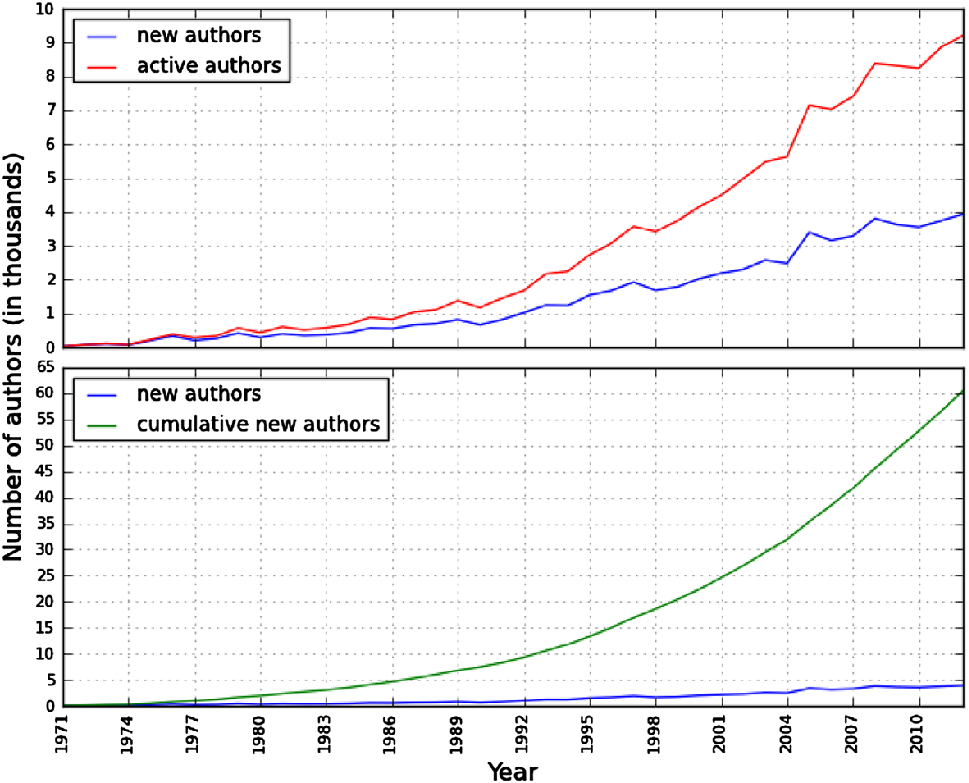
\includegraphics[width=\textwidth]{figures/fig-rise}
\caption{New and active authors in software engineering (1971\textendash2012) from DBLP,
for conferences and journals; (top) new and active authors; (bottom) new authors and
cumulative new authors. This figure comes from \citep{figurerise}.}
\label{fig:rise}
\end{figure}

Moreover, if the authors are disambiguated, the digital library can profit from exchanging
information about authors with other on-line services, such as ORCID.

In order to improve quality of services, some of the major digital libraries hire curators.
The curators' r\^{o}le consist mostly of manual enhancement of the data. They are a counterpart
of librarians in a digital world. One of the major challenges in their work is the correct
attribution of publications to researchers. It is not a simple task (see
\myhy{sec:unobvious}{1.3}), and it takes a lot of precious time of people whose knowledge is 
irreplaceable to the services offered by digital libraries. With the rise of the data
available in the system, the curators will have to put more effort into solving this task.
Having the authors disambiguated automatically, one can reuse the same algorithm in order to
disambiguate new entries and thus allow the curators to work on other crucial tasks.

Clearly, a proper author disambiguation creates big opportunities for the digital
libraries. It can enhance the usability of such services, extend the communication between
different digital libraries, save the precious time of scientists and expose the
relationship between publications and authors.

\section{Problem statement}

In order to understand the problem let us formulate underlying concepts:

\begin{itemize}
    \item \textit{publication} - a document that was written by
    authors. Every author has his own
    signature on the publication, thus a publication stores a set of
    signatures.
    \item \textit{author} - a person who authored (or co-authored) a publication.
    \item \textit{signature} - a unique set of information about unique author of the
    publication contained within the title page of it, usually between the title and the
    abstract. Not to be confused with a handwritten depiction of a name.
    Usually it consists of the author's full names, his affiliation, sometimes his e-mail
    and/or his address. However, in this work, in order to shorten the terminology, we will
    treat the whole publication as a part of the signature, i.e. having a
    signature the algorithm can deduct the signatures of co-authors, read the abstract,
    etc..
\end{itemize}

\begin{figure}[th!]
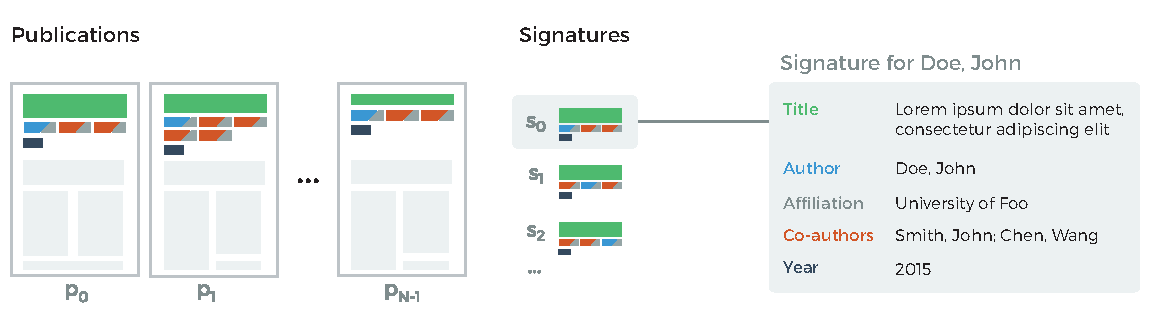
\includegraphics[width=\textwidth]{figures/fig-pub-to-signature}
\caption{An example signature s for "Doe, John" in a digital library environment.
A single publication contains a set of signatures. A signature
is not only the name of the author on the paper, but also the available metadata, such as:
the title of the publication, affiliation of the author, list of co-authors and the year of
publication.}
\label{fig:pub-to-signature}
\end{figure}

Formally, a digital library stores a set of publications ${\cal P} = \{ p_0, ...,
p_{N-1}\}$. Let us denote by ${\cal S} = \{ s, s \in p, p \in {\cal P}
\}$ the set of all signatures that can be extracted from all publications in ${\cal P}$.
Each signature belongs to one of the authors from  ${\cal A} = \{ a_0, ..., a_{M-1}\}$.

Author disambiguation can be stated as the problem of finding a
set of clusters ${\cal C} = \{ c_0, ..., c_{M-1} \}$ of ${\cal S}$ such that:
\begin{itemize}
\item{clusters $c_{1}, ..., c_{M-1}$ contain all of the signatures form ${\cal S}$ and none of the clusters overlap;}
\item{each subset $c_i$ (clusters) corresponds to the set of all signatures belonging to the same
individual $a_i$.}
\end{itemize}
Alternatively, the set ${\cal A}$ may remain (possibly partially) 
unknown, such that author disambiguation boils down to finding a partition ${\cal C}$
where subsets $c_i$  each correspond to the set of all signatures from the same
individual (without knowing who). Finally, in the case of partially annotated databases
as studied in this work, the set extends with the partial knowledge ${\cal C}^\prime = \{
c_0^\prime, ..., c_{M-1}^\prime \}$ of ${\cal C}$, such that $c_i^\prime \subseteq c_i$,
where $c_i^\prime$ may be empty.

In simple words, in order to perfectly disambiguate authors, for each author, we should
group together all his signatures, and only those.

\section{Non-obvious examples}\label{sec:unobvious}
In this section, we will show that disambiguation from a human perspective might be
a complicated task. We present few examples of signature pairs from the field of high
energy physics where it is far from obvious to tell whether they belong to the same author or
not. The answers come from the Inspire repository. In each example both signatures were
claimed in the Inspire system by curators or the author himself.

Every entry for a signature below is represented in a single frame and it contains the title
of the paper on the top. Below we included author's name as it appears on the paper, author's 
affiliation if it is available, collaboration for which the paper was written, experiment for 
which the paper was written, date of publication, category and keywords. Note that some 
additional metadata is available on Inspire. We decided to present here the data that is 
usually used by curators to decide who the signature belongs to. Each page contains a pair of 
signatures that requires disambiguation.

The reader is encouraged to try guessing if signatures from the examples belong to one
person.

\newcommand{\signatureexample}[9] {
\begin{framed}
  {\fontsize{14}{16}\fontseries{bx}\selectfont #1}\par
  % \textbf{Abstract:}\par #5 \par
  \begin{flushleft}
  \textbf{Author name:} #2 \par
  \textbf{Affiliation:} #6 \par
  \textbf{Collaboration:} #3 \par
  \textbf{Experiment:} #7 \par
  \textbf{Date of publication:} #4 \par
  \textbf{Category:} #5 \par
  \end{flushleft}
  \textbf{Keywords:}\par #8 
\end{framed}
}
\newpage

% Cytować?

\begin{center}
\textbf{Example 1}
\phantomsection
\label{ex1}
\signatureexample{Directed flow of anti-protons in Au + Au collisions at AGS}{G. Wang}{E877}{April 2000}{Experiment-Nucl}{not available}{BNL-E-0877}{scattering: heavy ion, gold, anti-p: particle flow, angular distribution: anisotropy, transverse momentum dependence, rapidity dependence, dependence: impact parameter, quantum molecular dynamics: relativistic, magnetic spectrometer: experimental results, Brookhaven PS, 11.5 GeV/c/nucleon}

\signatureexample{Quark transport properties in the region of coexistence of both hadronic and QGP phases}{Gang Wang}{none}{2001}{Phenomenology-HEP}{Harbin U. Sci. Tech.}{none}{quark gluon: plasma, matter: hadronic, quark: transport theory, soliton, color: space, spin: space, critical phenomena, numerical calculations}

\end{center}

These signatures belong to different authors. Although on the former signature only the
initial of the given name is available, we can tell that this paper was also written by
Gang Wang. A different one. As of 2015, Inspire database contained 4 profiles of
physicists named Gang Wang who actively used the portal.

\newpage

\begin{center}
\textbf{Example 2} 
\phantomsection
\label{ex2}
\signatureexample{Classical transport theory for a gluon plasma}{Gang Wang}{none}{2000}{Phenomenology-HEP}{Harbin U. Sci. Tech.}{none}{gluon: plasma, transport theory: classical, field equations, quark}

\signatureexample{Elliptic flow of non-photonic electrons in Au+Au collisions at $\sqrt{S_{nn}} =$ 200, 62.4 and 39 GeV}{G. Wang}{STAR}{May 24, 2014}{Experiment-HEP, Experiment-Nucl}{UCLA}{BNL-RHIC-STAR}{electron: elliptic flow, transverse momentum, correlation: two-particle, STAR, heavy ion: scattering, gold, correlation: (4particle), energy dependence, angular distribution: asymmetry, heavy quark: semileptonic decay, experimental results, Brookhaven RHIC Coll, 39.0: 62.4: 200.0 GeV-cms/nucleon}

\end{center}

These two signatures belong to the same author. Note that the affiliations and categories
of the papers are different. Both signatures belong to the author of the second signature
in the Example 1.

\newpage

\begin{center}
\textbf{Example 3}
\phantomsection
\label{ex3}
\signatureexample{The MAJORANA DEMONSTRATOR: A Search for Neutrinoless Double-beta Decay of Germanium-76}{R.A. Johnson}{Majorana}{Sep 2011}{Experiment-Nucl}{Washington U., Seattle}{none}{none}

\signatureexample{Constraining muon internal bremsstrahlung as a contribution to the MiniBooNE low energy excess}{R.A. Johnson}{MiniBooNE}{Oct 2007}{Experiment-HEP}{none}{FNAL-E-0898}{neutrino nucleon: interaction, neutrino/mu, charged current, muon-: leptonic decay, neutrino: oscillation, neutrino/e: particle identification, neutrino: energy spectrum, muon: bremsstrahlung, background, numerical calculations: interpretation of experiments}

\end{center}

Although both of these papers were written by people who are called R.A. Johnson, the former signature belongs to Robert A. Johnson and the latter to Randy Allan Johnson.

\newpage

\begin{center}
\textbf{Example 4} 
\phantomsection
\label{ex4}
\signatureexample{Effects of Limited Calorimeter Coverage on ET}{A.V. Vanyashin}{none}{Mar 1992}{Experiment-HEP}{SSCL}{none}{none}

\signatureexample{Search for single $b*$-quark production with the ATLAS detector at $\sqrt{s}=7$ TeV}{Alexandre Vaniachine}{ATLAS}{Jan 2013}{Experiment-HEP}{Argonne}{CERN-LHC-ATLAS}{interaction: chromomagnetic, p p: scattering, ATLAS, electroweak interaction, CERN LHC Coll, benchmark, dilepton: final state, final state: ((n)jet lepton), new particle: search for, bottom: excited state, excited state: decay, excited state: coupling, excited state: mass: lower limit, channel cross section: mass dependence, statistical analysis, experimental results, p p --> bottom anything, bottom --> top W, 7000 GeV-cms}

\end{center}

Despite the differences in surname spelling, this is the same author. This is an example for
different transliteration techniques.

In summary, having a pair of signatures it is often too hard to say whether the papers were
written by the same person or not. However, modern algorithmic techniques allow computers to
have deep insight into metadata offered by the digital libraries.

\section{Identifiers as an alternative approach}

Another solution emerging in the latest years involves identifying authors not by name, but
by unique, persistent identifiers. If all the authors used the same identifier system, and
they added their identifiers to their signatures, the problem of disambiguation would be
solved, as the authors would be simply referred to by their identifiers. The solution resembles
usage of Digital Object Identifiers in case of disambiguation of scholarly artifacts. One of
the most noteworthy and popular systems is
\textit{The Open Researcher and Contributor ID - ORCID} \citep{orcid}. The community behind
it aims not only to attribute persistent identifiers to the authors, but also it serves as
a storage to all the disambiguated signatures, offering a possibility of exchanging the data
between all the digital libraries involved in the project using the same API. Inspire is one of
the libraries that closely cooperates with ORCID on filling their database with correctly
disambiguated data.

One more system was used unsuccessfully in Inspire in the past. This approach was called
INSPIREID. The identifiers were assigned only to people who had their profiles on this
service. Comparing to current ORCID's solution this idea seems counterproductive.

Another system that is used even in wider context than science is ISNI \citep{isni}. This
standard offers identifiers that can be used by any entity, usually people or companies.

Unfortunately, despite the efforts aimed at dissemination of some identification systems for
people, the progress is slow. It will take many years to popularize the idea to the extent
where no other disambiguation is needed.


\chapter{Related work}\label{chap:related}

The problem described in this paper as author name disambiguation has been discussed in
many publications under various names. When applied to a broader domain or slightly modified,
it is often named as entity resolution \citep{Whang}, entity matching \citep{Kopcke}, record 
linkage \citep{Bhattacharya}, name matching \citep{Bilenko}, duplication elimination 
\citep{Ananthakrishna}, record deduplication \citep{culotta2007author},
\citep{bitton}.\footnote{Seeing this ambiguity, perhaps after solving the author name
disambiguation problem, we should work later on the problem of scientific domains
disambiguation.} Thankfully, the techniques presented in this work are versatile enough to
be adapted to all the mentioned problems with a little effort.

There were numerous attempts to tackle author disambiguation. The variety of the solutions
is caused by few factors:

\begin{itemize}

\item The richness of the metadata - some systems store only titles of the publications and the
authors names, when others contain very detailed metadata with keywords, affiliations,
references, citations and many more included.

\item The availability of the labeled data - some systems have an access to manually
labeled ground truth that can be used as training data.

\item The desired solution - some systems need to assign clusters to specific author
records, when others require only the correct clustering (i.e., the clusters need
not to be assigned to persons).

\item The range of the algorithm - some systems disambiguate only a part of the available
signatures.

\item Availability of curators - some systems have a possibility of fixing the outcome of the
algorithm if it contains incorrectly linked entities. Others need to be more strict, and might
prefer false negatives to false positives (i.e. they might prefer splitting signatures of an
author into multiple clusters than assigning signatures of multiple authors to one person).

\end{itemize}

Although the author name disambiguation problem was noticed and investigated in a publication
from as early as 1959 \citep{Newcombe}, multiple solutions burgeoned in the last ten years.
This is caused by the rise of the available data that is harder and harder to maintain
manually. Moreover, increased efforts to make web services more user-friendly resulted in
the demand for correctly linked records.

The theoretical definition of the record linkage problem was introduced in
1969 \citep{fellegi}. It is given as follows: 

\begin{quote}
The problem of recognizing
those records in two files which represent identical persons, objects or
events
\end{quote}

This definition, if applied only to the author names domain, is equivalent to the definition
of author name disambiguation presented by us.

In the last years the problem of author name disambiguation and the solutions were summarized
by few surveys, including \citep{Klaas}, \citep{smalheiser2009author} and
\citep{Ferreira:survey}.

\section{Unsupervised algorithms}

The publication of \citep{Newcombe} is of value as it indicates the problems that touch
every emergence of the disambiguation problem and it states that these can be best
overcome by an algorithmic solution, despite the weakness of the computation power of
those days. The solution in that work is based on the Soundex phonetic system, and it
does not require any labeled data.

Although supervised techniques gained popularity in the recent years, there are numerous
use-cases where they are not applicable. Usually it is caused by the lack of any training
data. In order to create an unsupervised algorithm, one needs to define a
handcrafted linkage function which represents the distance between two given signatures.
The most popular choices for similarity functions are mentioned in the work by Lee, On, Kang
and Park \citep{Lee}. These functions are:

\begin{itemize}

\item{Jaccard similarity \citep{Jaccard}}
\item{Jaro distance \citep{jaro}}
\item{Jaro-Winkler distance \citep{winkler}}
\item{Cosine similarity}

\end{itemize}

It is important to note here that originally Jaro and Jaro-Winkler distances were introduced
as a mean to solve the record linkage problem.

Let us shortly describe few interesting unsupervised approaches:

\begin{itemize}

\item{
Malin \citep{malin2005unsupervised} worked on disambiguating names in IMDB (Internet Movie Database) and used two different approaches. The first one used hierarchical clustering
\citep{ward1963hierarchical}, and used cosine similarity as the linkage function. His other
approach was to represent the network as a graph, and then traverse it with random walks.
The walks build probabilities that two records belong to the same author. Then, the edges with
probabilities below empirically set threshold are removed and the components of the graph
represent the final solution.
}

\item{
McRae-Spencer and Shadbolt \citep{mcrae2006also} proposed another graph-based approach.
The similarity graph was built in bottom-up fashion by applying iteratively few high-confidence
rules for signatures linking. Like in the Malin's publication the resulting components are the
clusters with authors.
}

\item{
Song, Huang and Councill \citep{song2007efficient} decided to solve the problem using
hierarchical Bayesian text models, such as Latent Dirichlet Allocation and Probabilistic
Latent Semantic Analysis, building them on the distributions of publications topics. Then,
having this models, they applied hierarchical clustering algorithm to cluster the signatures.
}

\end{itemize}

There are works that focus on different metadata fields available:

\begin{itemize}


\item{
Kang et al. \citep{kang2009co} based their solution on co-authors list stating that the
identity of the authors can be characterized only by the names of the people they wrote
publications with. The importance of the co-authorship attribute was corroborated by Fan
et al. \citep{fan2011graph}. Additionally this work uses an unusual clustering technique,
rarely seen in this problem - affinity propagation.

}

\item{
Schulz et al. \citep{schulz2014exploiting} focused on exploiting the citation
network and self-citations in addition to the co-authors list. 
}

\end{itemize}

Some of the library systems expose very limited metadata, such as author names and
publication titles, making the task harder. The task of author disambiguation with limited
metadata is sometimes called \textit{name disambiguation} and few solutions were presented by
Ferreira, Gon\c{c}alves and Laender \citep{ferreira2014disambiguating}.

The importance of author disambiguation for scientific world was highlighted by
data science contests, where the problem was approached from various perspectives.
One of the sources of non-disambiguated signatures data was \textit{Track 2 of KDD Cup}
\citep{kdd}. The winning team noticed that heuristic unsupervised algorithms should take
into account the origins of the author \citep{chin14a} as some features, especially names,
have emphatically different distributions and characteristics in the data depending on the
ethnicity. This algorithm splits the dataset into two subsets examined separately. One
contains only the Chinese authors, and the other the rest. Thanks to this observation, it
scored better than many sophisticated supervised solutions.

\section{Supervised algorithms}\label{sec:related}

%\item{
%Han, Zha and Giles \citep{Han03} used k-means algorithm \citep{macqueen} built on top of a Naive
%Bayes model and manually labeled data. The same authors used later spectral clustering for metadata
%containing co-author names, paper titles and publication venue titles \citep{Han}.
%}

In order to evaluate heuristic algorithms mentioned in the previous section, digital
libraries had to create datasets with correctly labeled signatures. The labels were
usually gathered with close cooperation with the authors.
On the other hand, some digital libraries (e.g.
\textit{Inspire}) implemented functionalities allowing users to take an active part in
curating scientific databases.  Both of these approaches led to the rise of the training
data that could have been used as training data in supervised algorithms.

Even when there is no labeled data available, and the authors have no intentions of
curating the data on their own,
supervised approaches can be implemented. Levin, Krawczyk, Bethard and Jurafsky 
\citep{levin2012citation} bootstrapped the training data using high confidence
linking function. Although this technique can lead to mislabeled training data,
the solution proved to be more accurate than unsupervised techniques.

The popular approach, considered to be state-of-the-art these days, consists of two steps. 
Firstly, a classifier determining whether two signatures were written by the same person is 
trained. Then, this classifier is used as a distance function (called also \textit{linkage 
function}) during the clustering phase, which should output sets of signatures belonging to 
separate authors.

However, there are cases where there is too little data to create an accurate classifier. This was 
often dealt with by creating semi-supervised strategies that attempt to gain the advantages of 
manually created empiric linkage functions with machine learning techniques applied to smaller 
datasets. This solution is often applied on automatically
extracted training data, showing a way to outperform unsupervised strategies 
\citep{ferreira2010effective}, \citep{torvik2009author}. It is important to note that the
labeled data can be useful in both linkage function learning and clustering steps.
For example, \citep{levin2012citation} use this data to prevent clustering together signatures
from different authors after learning a logistic regression classifier.

When the number of authors is small another approach was to use a multiclass classifier
which learns directly which author the signature belongs to. There is a significant number
of algorithms tried:

\begin{itemize}

\item{Han et al. \citep{han2004two} tried Na\"{i}ve Bayes and SVM.}
\item{Clotta et al. \citep{culotta2007author} used ranking perceptron.}
\item{Treeratpituk and Giles \citep{treeratpituk2009disambiguating} tried random forests
and they noticed they feature importance output by the trees \citep{louppe2013understanding}
can be a high-quality method of choosing features to eliminate.}
\item{Finally, deep neural networks have been tried with satisfactory results
\citep{tran2014author}.}

\end{itemize}

Among the proposed two-step supervised solutions there is no consensus on the classifier for 
the linkage function and the clustering algorithm. For example, Huang, Ertekin and Giles
\citep{huang2006efficient} used LASVM and DBSCAN, while \citep{levin2012citation} tried lasso logistic regression
and hierarchical clustering.

Coming back to the \textit{Track 2 of KDD Cup}, some of the top solutions used supervised
techniques. The team that ended up on the 7th position decided to create empirically a training
set, and then use supervised techniques \citep{Zhao:2013}. It shows that even when there are no
labels in the dataset, it might be worth to introduce some. Thus, when a large labeled dataset
is available, supervised approaches should perform better than handcrafted heuristics.

One of the problems that supervised algorithms need to overcome is the imbalance between the 
labeled and unlabeled signatures. The rising amounts of the data available in digital 
libraries makes the large coverage of the signatures with labels hard to achieve. Simple 
statistical evaluation of an algorithm can be inaccurate due to vast differences between labeled 
and unlabeled data.

It is important to note that the solution to the author disambiguation problems should be tailored 
to the environment in which it will be used. This consists of: amount of the labeled data available, 
richness of the metadata, the distributions of specific features and the domain of the digital 
library \citep{santana2014combining}.

The labeled data used in the mentioned solutions was rarely publicly released and when it was
released, the datasets were small or too domain specific. Hence, the algorithms 
described in this chapter could not be directly compared. As there is a need for a common
benchmark, we released the first large labeled set of signatures that is used in this
work \citep{Louppe}.

\section{Associated problems}

Working with large datasets might create a computational problem. The clustering
algorithms usually have at least square time complexity. The algorithms that are faster
(like Birch algorithm) have their limitations that make the applications of them
tough. For example, the Birch algorithm requires information about the desired number
of clusters which is not available in our case. In order to overcome the computational issue, the
signatures might be initially \textit{blocked} \citep{On}. Blocking is a pre-clustering
step that aims to split (i.e. partition) the initial set of the signatures into smaller 
chunks without splitting signatures belonging to the same authors.

Disambiguation of the whole dataset takes a lot of time and should not 
be rerun when the new data arrives. In the desired scenario, the disambiguation should be 
incrementally expanded over the new signatures. There are various aspects that have to be 
considered here. The new signatures can indicate that two clusters from the previous 
disambiguation should be merged. This is dealt with in the paper by Esperidi{\~a}o et al. 
\citep{Esperidiao}. Interesting approach was taken by Qian et al. \citep{qian2015dynamic}.
They propose a probabilistic model for each existing cluster that predicts if a new
publication was written by a given author. When a new publication arrives, their solution is
able to merge clusters or create new clusters if necessary. Moreover, they claim that their
solution has lower computational complexity than other incremental clustering algorithms like
incremental DBSCAN \citep{ester1998incremental}.


\chapter{Overview of techniques}


In order to introduce the reader to the proposed solution, we present the theoretical background
for the algorithms used in this work.
We will describe feature processing techniques, classifiers and the clustering used further.

\section{Training data preparation}

In order to perform any algorithmic task, we need to model the input data. When available
metadata consists of numbers, the preprocessing step does not require any sophisticated
techniques. For example, the comparison of the publication years might help the
classifier. An author is not expected to publish two papers separated by 70 years, but it is
quite probable that his papers are few years apart. Then, the
difference between two compared papers is a meaningful and easy to construct feature.
However, some of the metadata fields available in the Inspire system store text data and
it is far less obvious how can that information be processed by an algorithm.

Let us divide text fields into two types:

\begin{itemize}

\item{\textit{categorical text field} - a field that classifies a publication into multiple
categories. An example is the \textit{keyword} field. The categories are the keywords and a
publication might be associated with several of them.}

\item{\textit{descriptive text field} - a field that contains a description of an entity. A good
example is the \textit{abstract} field - a block of text that summarizes a publication}

\end{itemize}

We will provide means to create vectorized representation of these fields and then we will
discuss how to meaningfully measure similarity between these vectors.

\subsection{TF-IDF}

Let us firstly mention that we can divide any text field into tokens. For categorical text
field an obvious way to do that is to use each category as a single token. In case of
descriptive fields, we can treat each word present in the field as a token. Now, in order
to compute similarity, one could
think of a na\"{i}ve approach where it is measured using only information available
in the fields compared. For example, one could compute the number of words occurring in
both of the compared abstracts and divide it by the sum of the number of words in these
abstracts. Such function would reach 1 if the abstracts are the same and 0 if they do not
share a single word. However, this function does not reflect the similarity well, as different
words have different occurrence frequencies. A better approach should take into
account the importance of each token from the field. A widely used solution is called
TF-IDF \citep{Salton1983}.
It consists of the normalized term frequency (TF) divided by the inverse document frequency
(IDF). Here, the term \textit{document} denotes a single text field. 

Term frequency measures how often a token occurs in a document. In our case, this
frequency is divided by the total number of words in the document in order to provide
normalization.

Inverse document frequency measures how insignificant the token is among all documents
considered. The tokens that appear often (like word \textit{we} in abstracts) do not
carry a lot of useful information - they can not tell us a lot about similarity of two
documents - and thus have to be scaled down. This is achieved by dividing the TF by the IDF.
The formula for the IDF is:

\[ IDF(\textit{t}) = \ln(|\text{documents}|/|\text{documents containing \textit{t}}|) \]


One could argue that this does not lead to the perfect similarity function, as during
this preprocessing step the semantic meaning is lost. In recent years some vectorization
approaches with semantics recognition were developed \citep{word2vec}. In this work, these
novel techniques are not discussed.

\subsection{N-grams}

In some situations an improvement over a standard TF-IDF can be achieved with finer
granularity of token. For example, in case of names in a digital library, sometimes
typos are present in the data. A trivial approach of modelling the \textit{Full name}
field in the model with TF-IDFs treating each word as a single token would penalize
typos heavily. Instead, we can take care of the situation where long tokens are similar
by splitting the tokens into small pieces. Such a piece is called an $n$-gram, where $n$ is
the length of it. For example, we can create $3$-grams of the token \textit{Jones}. The resulting
$3$-grams will be: \textit{Jon}, \textit{one}, \textit{nes}.

In order to further improve the sensitivity of the resulting TF-IDF vectors, instead of
considering only fixed length $n$-grams, we can broaden the domain by adding shorter/longer
$n$-grams to the documents.

\begin{mydef}
The $(m,n)$-gram of a token where $n > m$ is defined as the sum of m-grams, m+1-grams, ... , n-grams
over this token.
\end{mydef}

\subsection{Vector similarity functions}

Having vectors that represent text data, we can use simple mathematical functions in order
to measure the information shared by them. The functions commonly used for text fields
are:

\begin{itemize}

\item Jaccard similarity \citep{Jaccard} - $f(\vec{x},\vec{y}) = \frac{\sum_{i}{min(x_{i}, y_{i})}}{\sum_{i}{max(x_{i}, y_{i})}}$

\item Cosine similarity - $f(\vec{x},\vec{y}) = \frac{\vec{x} \cdot \vec{y}}{\lVert \vec{x} \rVert * \lVert \vec{y} \rVert}$

\end{itemize}



\section{Supervised learning}

In a supervised learning problem one has a set of labeled data, that is, input-output 
value pairs. The labeled data is often called \textit{training data} and it consists
of \textit{training examples}. The task is to learn a function using the training data 
which will generalize well on new examples, i.e. will correctly predict the output for
the new examples. In evaluation benchmarks the new examples are called \textit{test data}.

Using mathematical notation, the task is to find a function (it is often called \textit{model})
$\varphi: X \rightarrow Y$, where $X$ is the input space and $Y$ is the output space.
The training data is a set of training examples:
$(x_{1}, y_{1}), (x_{2}, y_{2}), ..., (x_{n}, y_{n})$ and each of them is a vector of attribute values. The attributes
are often called \textit{features}. A feature might be
\textit{quantitative} (\textit{numerical}) or \textit{categorical}. When a feature is
numerical, each of its values is a real number. When a feature
is categorical, each of its values is an element of a finite set of any type.
For computational simplicity, the categorical features are usually projected into the space
of integer numbers. The dependent attribute is a vector $y_{1}, y_{2}, ..., y_{n}$ which elements
can be real numbers (then the prediction task is called \textit{regression}) or can come from a finite 
set (then the task is called \textit{classification}).

In this framework, the training data is a set of pairs $(x_{1}, y_{1}), (x_{2}, y_{2}), ...
(x_{n}, y_{n})$ where $\forall_{i=1,...,n}: x_{i}\in X \wedge y_{i}\in Y$. The test set (i.e. test data) is
another set of pairs $(x_{t}, y_{t})$ used for evaluation of the model. 
The training set and test set should not overlap and the model should not have an access to
the test data while it is trained.

In order to know if the prediction is useful, such algorithms are evaluated on the test set
using some function $L: X \times Y \rightarrow \mathbb{R}$, called often
\textit{loss function}. Put otherwise, the task is to minimize \textit{generalization error}
on the test set. In machine learning, there is an assumption made that the distributions of the training set
and the test set are similar. The algorithms able to learn models are called
\textit{classifiers}.

As machine learning models have no access to the test set during the training phase, it is
easy to create a model that has no error on the training set, but does not generalize well
to the test data. This is an extreme example of what is called \textit{overfitting}. 
Overfitting is a situation where a complex model describes noise in the training data
at the expense of describing the actual relation between $X$ and $Y$.
Many models offer possibility of taming overfitting by setting additional \textit{regularization} terms.

\section{Discriminative linear classifiers}

Popular classifiers for learning models with linear dependencies
base on the idea of finding a hyperplane that separates two classes of the examples from the
training set in the best way. The difference between various discriminative classifiers is
drawn by the way how they define the best separation. Although these classifiers are not
able to discover non-linear dependencies, one can project the input space in such
a way that the hyperplanes determine non-linear boundaries after projection reversal.
This method is called \textit{kernel trick}.

Although a single hyperplane can help us only with binomial classification, it is easy to extend this
method to the multinomial problem. The most popular solution is called \textit{one-versus-all}
classification scheme. It is a scheme that runs the training procedure linear number of times
with regards to the number of classes. For each class, it learns a classifier that separates
this class from the rest of the examples. Then, each example is classified to the class
for which the corresponding classifier reported the highest confidence out of all the
classifiers.

\subsection{Linear regression}

In the task of regression linear classifier finds vectors $A$ and constant $b$ such that
$L(A\vec{X}+ b, Y)$ is minimized. Usually this is done by minimizing \textit{least squares}.

\begin{mydef}
Least squares optimization problem for model $m$ is defined as:
\[min_{x_1\dots x_T} \sum_{i=1}^{n} (y_{i} - f(x_{i}))^{2}\]
\end{mydef}

Linear regression has been a popular choice for data analysis performed on small datasets
due to its simplicity. Often it is applied to data with high-dimensionality problem.

\subsection{Support Vector Machine with a linear kernel}

Sometimes, in the classification task, we would like to not only classify correctly training
examples, but also classify them with the highest possible confidence. Let us consider an example
where the training data is linearly separable. Then,
it is possible to select two parallel hyperplanes such that they separate the classes and
the space between them does not contain any examples.
In this case the Support Vector Machine (SVM) maximizes the distance between
the hyperplanes. We can think of the distance between the hyperplanes as the
confidence level. Let us denote hyperplane as $\vec{w}*\vec{x} - b = 0$ where $\vec{w}$
is the normal vector to a hyperplane separating the classes. The $b$ parameter
can be thought of as the distance from the hyperplane to the nearest points.

\begin{mydef}
Support vector machine problem with a \textit{hard-margin} is defined as:
\[min_{\vec{w}} \left\lVert{\vec{w}}\right\rVert\]
subject to:
\[y*(\vec{w}*x -b) \ge 1\]
\end{mydef}

As data tends to contain some noise, all of the training examples
might not be linearly separable. Then, a regularization term is added to the formula.
Additionally, the minimized loss function is the hinge loss.

\begin{mydef}
Hinge loss function is defined as:
\[l(z) = max(0,1-t * z)\]
\end{mydef}

\begin{mydef}
Support vector machine problem with a \textit{soft-margin} is defined as:
\[min_{\vec{w}}\Bigg[C\sum_{i=1}^{n}max(0, 1 - y*(\vec{w}*x -b))\Bigg] + \frac{1}{2}\left\lVert{\vec{w}^{2}}\right\rVert\]
\end{mydef}

The \textit{C} parameter is an example of a regularization term. For large values of \textit{C} the
optimization will prefer the hyperplanes that correctly classify larger number of samples but
do not necessarily preserve the idea of large separation margin. The
smaller values of \textit{C} will promote the hyperplanes that keep separation margin large, but
might misclassify many training samples in case of noise. With \textit{C} set to zero the 
soft-margin SVM is equivalent to hard-margin SVM.

SVMs are a mature idea \citep{VapLer63}. They were often treated in the past as black boxes
as they give satisfactory result without fine tuning.


\section{Decision trees}
One of the most widely used classifier is the decision tree \citep{quinlan1986induction},
\citep{morgan:1963}.
It is a tree that stores a decision (rule) in each of its nodes.

\begin{mydef}
 A tree is a graph $G = (V, E)$ where any two vertices are connected by a single path.
\end{mydef}

\begin{mydef}
 A rooted tree is a tree where one of the vertices is designated as a root.
\end{mydef}

\begin{mydef}
 A binary tree is a rooted tree where all internal nodes have exactly two children.
\end{mydef}

The whole tree represents the classification
process. Whenever a new example needs to be classified, it traverses the tree starting at the
root. In each node, the attributes of the new example are compared with the rule in the node
and a decision is taken which branch to follow. The leaves determine the output classes, thereby
when a new example ends its route, a class is assigned to it. In machine learning,
due to computational and representational simplicity the decision trees are usually
binary.

Decision trees are built in top-down fashion. During the building process, the leaves are
associated with some training examples that previously traversed the path to the given leaf.
The procedure starts with a tree containing only one vertex and all the examples from the training set.
Whenever we want to expand a leaf, an attribute that makes the "best" split is chosen,
and a new decision rule is created. The training examples are split over the rule and they are
assigned to the new leaves. The best split is usually defined as the split that creates the
biggest possible information gain. Adding a new leaf can 
be interpreted as a division of the prediction space. If the task to solve is regression,
the split minimizes the squared error loss, and the leaves annotate the values from 
$\mathbb{R}$.


\begin{figure}
\begin{subfigure}[b]{.4\textwidth}
    
    
\centering
    \resizebox {\linewidth} {!} {
        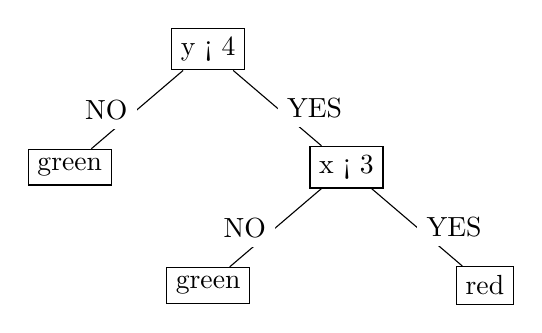
\begin{tikzpicture}[sibling distance=10em,
          every node/.style = {shape=rectangle,
            draw, align=center,
            top color=white, bottom color=white}]]

          \node {y < 4}
            child { node {green} edge from parent node[left,draw=none] {NO} }
            child { node {x < 3} 
              child { node {green} edge from parent node[left,draw=none] {NO} }
              child { node {red} edge from parent node[right,draw=none] {YES} } edge from parent node[right,draw=none] {YES} } ;
        \end{tikzpicture}
    }


\vspace{1cm}

\end{subfigure} %
\begin{subfigure}[b]{.6\textwidth}

\centering
    \resizebox {\linewidth} {!} {
        
        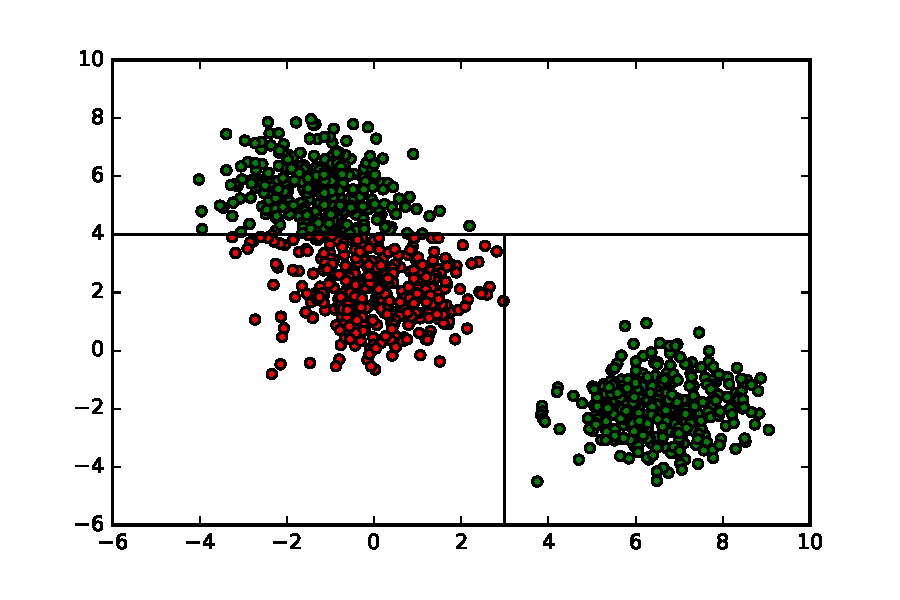
\includegraphics[width=\textwidth]{figures/decision-hiperplanes}
    }
\end{subfigure}
\caption{An example of a decision tree (left) classifying objects to two colors
and corresponding partition of $\mathbb{R}^2$ space with examples (right).}
\label{fig:tree}
\end{figure}

Decision trees have some advantages:

\begin{itemize}
\item{A tree is an easy to analyze and very self-explanatory
model. A single path from the root to the leaf can be interpreted as an implication. If all
the rules on the path are met by any example, this example probably belongs to the class
from the leaf.}
\item{They can handle heterogeneous data}
\item{They are fairly robust to outliers}
\item{By using trees one can discover which features are relevant. 
For example if a feature does not contribute to any rule in the tree, it is simply an
irrelevant noise that can be removed from the data.}
\end{itemize}

In case of the trees it is easy to overfit. For example, one can build a tree that
is too large. Due to noise in data and lack of representative instances, such tree
will not generalize well on new examples.

The decision trees are used in the regression problem as well. In this case, the
leaves do not contain the class name. Usually they store the average of the values from
the examples belonging to it. The average is updated whenever a new example is added to
the node. The node is split when the node impurity exceeds a set constant. This
technique for regression can be applied within any method that uses multiple decision
trees.

The exact algorithm for decision trees construction used in this work is Classification
And Regression Trees \citep{cart84}.

\subsection{Random forests}
Decision trees proved to be very powerful when they are fit
with some random perturbations to training data, and combined together. This
approach is called \textit{ensembling}. The aim is to create many decorrelated trees. One of
the most commonly used method from this family is called \textit{random
forest} \citep{breiman2001random}. The idea is to sample few subsets of training data and
construct a decision tree for each of them. The trees however also make use of randomness. During
the construction, when a leaf is expanded, only few random features are used to choose the
best split. The number of examples in the selected subset should be a small fraction of all
examples. A good starting size is the square root of the number of all examples.

Having many decision trees $(\varphi_{1}, \varphi_{2}, ..., \varphi_{m})$ trained on subsets
of the data, we need a way to combine their results and create a new prediction model
$\psi$. The simplest approach is to use a majority voting scheme. 

\begin{equation}
\psi_{\varphi_{1}, \varphi_{2}, \ldots, \varphi_{m}}(x) = \underset{c\ \in\ Y}{\operatorname{argmax}}\sum_{i=1}^{m}  \mathbbm{1}(\varphi_{i}(x) = c)
\end{equation}

However, if the trees provide class probabilities $p$ for the output, a smoother approach is to
use \textit{soft voting}. Soft voting takes into account probabilities of all the
classes and the returned value is the weighted average probability:

\begin{equation}
\psi_{\varphi_{1}, \varphi_{2}, \ldots, \varphi_{m}}(x) = \underset{c\ \in\ Y}{\operatorname{argmax}}  \frac{1}{m} \sum_{i=1}^{m} p(Y_{test} = c| X_{test} = x)
\end{equation}

\section{Boosting}
There are machine learning methods that use multiple classifiers and are applicable not only
to decision trees. One of the proven methods appears to be \textit{boosting} \citep{freund99ashort}. The 
idea is to fit the models sequentially and update the final classifier in each iteration
with the new prediction.

\subsection{Gradient Boosted Regression Trees}
In recent years, the most proven solution is called \textit{gradient boosting} \citep{friedman2001greedy}. To understand how it works let us denote:

\begin{itemize}
\item $F_{j}$ - the model created by the $j$-th iteration of gradient boosting
\item $G_{j}$ - the classifier added to the model in $j$-th iteration
\item $h$ - the hypothesis that would perfectly compensate $F_{j}$, i.e.
$\forall{i} F_{j}(x_{i}) + h(x_{i}) = y_{i}$ 
\end{itemize}

Using a simple classifier the target is to create $G_{j}(x) = F_{j}(x) + h(x)$. As
$h$ is not known, the classifier tries to minimize the loss on $y - F_{j}(x)$.
Usually, the \textit{shrinkage} technique is used as an addition in order to
generalize better. If the shrinkage parameter is denoted as $\upsilon$,
a single iteration of gradient boosting can be denoted as:

\begin{equation}
F_{j+1}(x) = F_{j}(x) + \upsilon * G_{j}(x)
\end{equation}

The shrinkage parameter should be set to a low value (for example, 0.001). If the
classifiers  used within the gradient boosting procedure are weak (i.e.
there are slightly better than a random prediction, but still inaccurate)
\citep{schapire1990thestrength} this approach tends not to overfit. The gradient boosting
procedure is typically used with shallow decision/regression trees.

\section{Artificial neural networks}
Another approach to supervised learning was inspired by the observation of biological
nervous systems. A single neuron can be represented as a simple mathematical model,
thus laying foundations to the imitations of brain. Artificial neurons, when combined
into networks, proved to be the state-of-the-art classifiers in many applications, such
as image recognition, sequence prediction and many others.

In order to understand how a neural network works firstly we should understand a neuron
and its artificial counterpart. Despite the fact that the current state of
neurobiology does not explain the whole process of human cognition, there is a
consensus \citep{PNS} over its basics. It is known that every typical neuron is an
electrically excitable cell which can process and pass electrical signal.
Neurons are subject to the \text{all-or-none}
principle. If the incoming signal is strong enough to be passed, the response
is always complete and keeps the same level of intensity.

Knowing that, one can notice that it is easy to express a neuron as a mathematical
model \citep{McCulloch1943}. Let the artificial neuron have $m + 1$ inputs $x$ indexed
from zero and one
output $y$. The signals will be expressed as values $0$ or $1$. Let us note
that the first input will always propagate a value of $1$ and it will be called
\textit{bias}. The other inputs come from other neurons (or input), and the
signals from them can be freely changed with constant weights $w$. Using a sum
operation over all the inputs, such a model can express a huge variety of functions.
Then, the sum is passed through the \textit{activation function} $\psi$ in order to produce 
an output. The work of a neuron can be expressed as a single formula:


\begin{equation}
y_k = \psi\bigg(\sum_{j=0}^{m}w_{kj}x_{j}\bigg) 
\end{equation}

A single neuron has its limitations which were thoroughly discussed
by Marvin Minsky and Seymour Papert \citep{Min69}. This publication diminished
the popularity of such solutions for the next twenty years. Fortunately, more recent
developments show that it is possible to learn complex function on high dimensional
domains if the neurons are integrated into a bigger system, a network. Usually
the artificial neural networks consist of layers. In this paper we will
analyze only fully connected layers, i.e. if we consider two consecutive layers,
every neuron in the former has a single output for every single neuron in the latter
(Figure \ref{fig:fig31}).
Such structure is often called multi-layer perceptron (MLP).
The most common type of artificial neural network consists of three groups of layers:

\begin{itemize}
    \item input layer - the first layer that represents the raw input that will be
    processed by the network
    \item hidden layers - a single hidden layer joins other two.
    \item output layer - the last layer that takes the output of another layer
    and outputs the result of the algorithm
\end{itemize}



\begin{figure}[H]
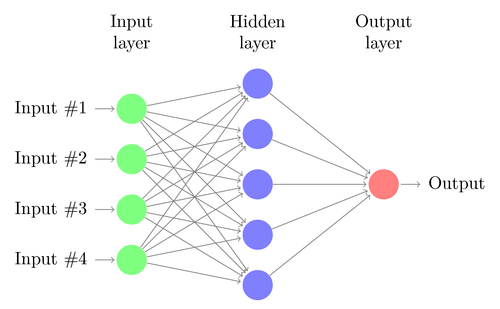
\includegraphics[width=\textwidth]{figures/fig31}
\caption{Graphical representation of a Multi Layer Perceptron. Each blob
represents a neuron.}
\label{fig:fig31}
\end{figure}

We stated that a large neural network can represent complex functions. In
the task of machine learning such function should correctly show the relationship
between the feature space and the output. The learning
procedure uses so-called back-propagation algorithm. This algorithm computes
the error derivatives of the weights. To do that, firstly, the rate at which the error
changes as the activity level of a unit is changed is computed. For example, for the
output layer it is the difference between the current prediction (the signal
received by running the network over the input sample) and the truth value. The
error derivative can be then computed by taking the product of this rate and the
incoming signal. The name of the algorithm comes from the fact that this derivative
is computed starting from the last layer in direction of the input layer.

A question to resolve is the choice of the activation function. There are different
approaches, however, in recent years the rectified linear unit (ReLU) function is
getting a lot of attention, as it allows the network to represent a non-linear function:

\begin{equation}
f(x) = max(0,x)
\end{equation}

In this work, in order to prevent overfitting of neural networks, we will use the dropout
technique \citep{dropout}.For each neuron in the layer, with some set probability,
this regularization technique disactivates the neuron, i.e., the neuron passes 0
further regardless of the input. This procedure imitates the ability of human brain to
transfer the functionality of damaged neurons to unused ones.

\section{Clustering}
In the task of unsupervised learning one of the objectives is to divide the solution 
space  into clusters. Basing on the relationship between examples, the clustering
algorithms derive the structure out of unlabeled data. The term cluster is hard
to define rigidly, as there are various approaches. In this work, we will treat
our clustering problem as a \textit{clustering with strict partitioning}.
Within this definition, a cluster is a set of objects that are more similar to each
other than to objects in other clusters. A single object must belong to exactly
one cluster. The number of the clusters can be
chosen arbitrarily, but some of the algorithms can suggest the preferable value by
examining the distribution models or by analyzing the densities of the subspaces.

Usually the input of such algorithms is the linkage function $d$ that defines the
distance between two examples. The evaluation method of such algorithm depends on the
application.

\section{Agglomerative hierarchical clustering}
One of the ideas for the clustering algorithms is to build clusters hierarchically. This means
that the set of all examples can be perceived as a single cluster, and every single example can be a single
cluster as well. The algorithm merges the clusters in the bottom-up fashion
(\textit{agglomerative clustering}) until a single cluster is left
\citep{ward1963hierarchical}, or split the clusters into smaller ones starting from the 
biggest (\textit{divisive clustering}). The splits or divisions are made in a greedy manner.

For the task of author disambiguation the more interesting algorithm is the agglomerative
clustering. It is cheaper computationally ($\mathcal{O}(n^{2})$) in some cases, and the
biggest advantage of divisive clustering - its ability to read the global patterns - does not
play a big role in our problem.

The agglomerative hierarchical clustering works iteratively. In each iteration it finds
a pair of clusters that minimize the \textit{linkage criterion} - the function
that defines the distance between clusters (let us denote them as $A$ and $B$). There are
multiple choices for the linkage criterion, and the most popular are:

\begin{itemize}
\item Complete linkage - $max \{d(a,b): a \in A, b \in B\}$
\item Single linkage - $min \{d(a,b): a \in A, b \in B\}$
\item Unweighted pair group method with arithmetic mean (UPGMA) \\
\citep{sokal1958astatistical} - $\frac{1}{|A|*|B|}\sum_{a \in A}\sum_{b \in B}d(a,b)$ 
\item Weighted pair group method with arithmetic mean (WPGMA) \\
\citep{sokal1958astatistical} - $d(S,B) + d(T,B)$ where $S$ and $T$ are the clusters
that created cluster A. This methods effectively creates an ultrametric tree.
\item Unweighted pair group method with centroid (UPGMC) \\
\citep{Sneath-Numerical-1973} - $\left\lVert c_{a} - c_{b}
\right\rVert_{2}$ where $c_{a}$ and $c_{b}$ are centroids of clusters $A$ and $B$
respectively. New centroids are computed using all elements of a cluster.
\item Weighted pair group method with centroid (WPGMC) \\
\citep{Sneath-Numerical-1973} - same as above, but new centroids
are computed using the centroids of joined clusters.
\end{itemize}

Another advantage of the hierarchical clustering is that it is easy to interpret. Often,
if the analyzed data is small, it is represent as a \textit{dendogram}. Dendogram
is a binary tree in which the examples are represented as leaves and each node represents
a cluster in a clustering.

\begin{figure}[!ht]
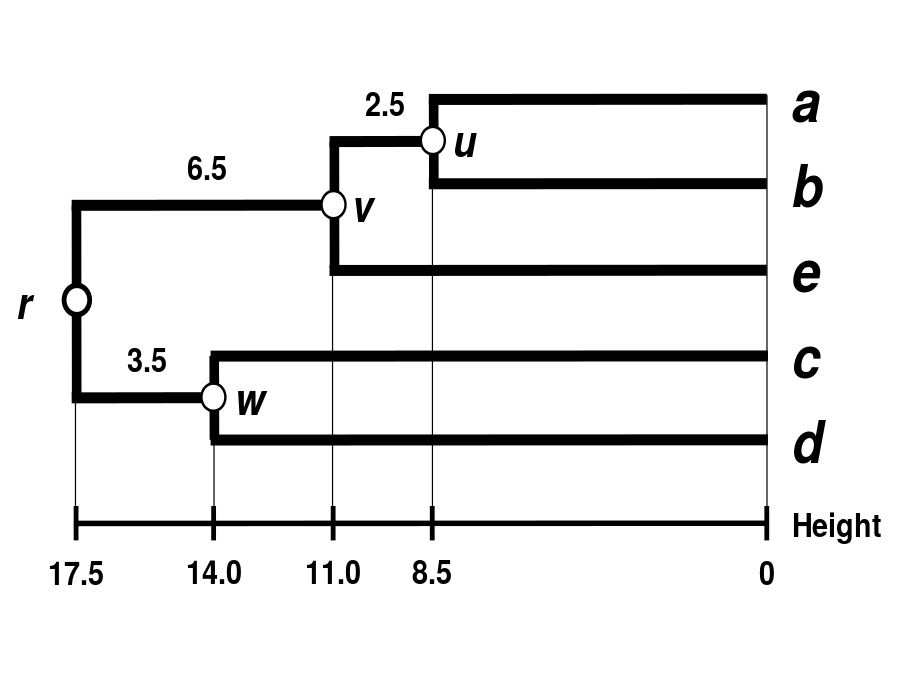
\includegraphics[width=\textwidth]{figures/Dendogram}
\caption{An example of a dendogram. The x axis represents distance between nodes. Each node
can be interpreted as a cluster. Cutting the tree with a straight cut parallel to the $y$ axis
can be interpreted as a clustering. For example, a cut on height $15.0$ represents a
clustering with two clusters: $v$ and $w$. The $v$ cluster consists of three signatures: $a,b$ and $e$.}
\label{fig:den}
\end{figure}

\section{Semi-supervised hierarchical clustering}
In some situations it is possible to enhance the clustering algorithm by using supervised
strategies. The method of interest to us uses partially labeled data, and thus it
belongs to the family of semi-supervised solutions.

After running hierarchical clustering algorithm, one needs to decide which partition
defines the result clusters. If we represent the clustering as a dendogram, this can
be done by cutting the tree. Without any labeled data, the best approach is to
set a threshold and accept merges only where the value of the linkage criterion was smaller
than it. This setting might be sub-optimal. However, having partially labeled dataset, one can
optimize some accuracy score when he decides which threshold to choose.

\part{Solution}

\chapter{Algorithm}
In this chapter, we will describe the solution implemented for the Inspire project.
As mentioned previously, the algorithm consists of three steps:

\begin{enumerate}
    \item Blocking
    \item Linkage function learning
    \item Clustering
\end{enumerate}

The whole process is illustrated in Figure \ref{fig:workflow}. 

\begin{figure}[!ht]
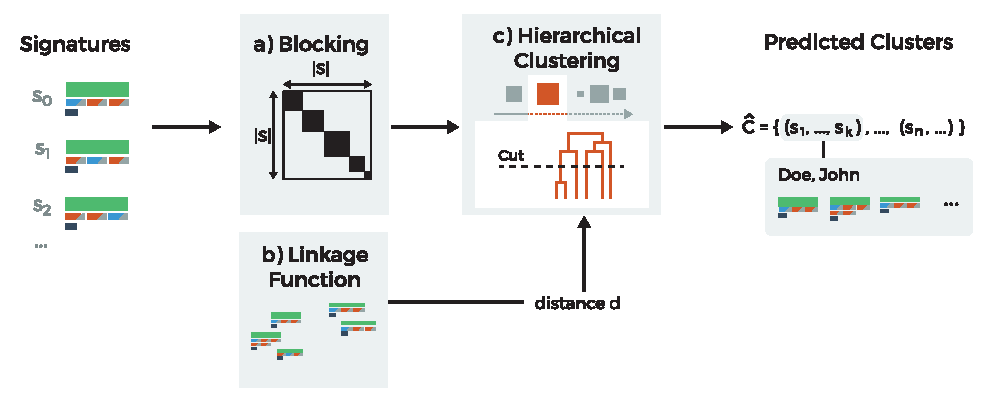
\includegraphics[width=\textwidth]{figures/fig-workflow}
\caption{Pipeline for author disambiguation. $s_{i}$ is a signature, $S$ - set of 
all signatures, $\widehat{\cal C}$ are the predicted clusters. The resulting clusters
are produced by the clustering step. In order to perform clustering, the linkage
function is needed. In order to reduce computational complexity the initial set of
signatures should be blocked before clustering.}
\label{fig:workflow}
\end{figure} 

\section{Blocking}
The labeled dataset used in this work consists of 1,201,763 signatures. Moreover,
in the real life scenario the disambiguation needs to be performed over all signatures,
including the unlabeled ones. The number of all signatures in Inspire reached 9 millions
in 2015 and constantly grows. As mentioned previously, the last step of our
algorithm is clustering. The clustering algorithms popular nowadays can be performed
in $\mathcal{O}(n^2)$ time. With 9 millions signatures to disambiguate, the cost
of computing the similarity that many times would cause the algorithm to run over
weeks.

In order to prevent this, the signatures can be \textit{blocked}.
The term is not very appropriate,
as a block is simply a single subset from the partition of the whole set of signatures.
Perhaps the term \textit{partitioned} would be more accurate, but in the domain of author
disambiguation the term \textit{blocked} was widely used \citep{fellegi, On,
huang2006efficient, levin2012citation} and we will stick to it in this paper.

Blocking is a technique that is used in every application of author disambiguation
that has to run on bigger datasets. The good blocking should on the one hand
minimize the number of signatures belonging to the same author split over multiple
blocks (so that they can be clustered together further in the algorithm), and on the
other hand reduce the number of operations that have to be performed during clustering.
Moreover, it is possible that clustering will be more precise when run on smaller
blocks, but given the complexity of the algorithm (the clustering's input are the
similarities produced by the classifier used in the linkage function step), it is
impossible to tell that without empirical results.

Blocking makes it possible to decrease the computational complexity in the clustering step
from $\mathcal{O}(n^2)$ down to $\mathcal{O}(\sum_{b} n_b^2)$ where $n_b$ is the size
of $b$-th block. Clearly, the smaller the blocks are, the less computations have to be
done. On the other hand, blocking can decrease the possible maximum recall achievable
by the algorithm. No matter what the resulting blocks are, it is possible to
theoretically achieve 1.00 precision by performing perfect disambiguation on single
blocks. But if two signatures belonging to the same author belong to two different
blocks, the value of recall of the algorithm will be smaller than 1.00. For the definitions of
precision and recall, see \myhy{sec:evaluation}{Section 9.1}

The possible improvements in this step were not thoroughly investigated. The most
widely used technique was blocking with \textit{sorted neighbourhood} scheme
\citep{Hernandez:1995:MPL:223784.223807}. The schemes used often were:
\begin{itemize}
\item The same last name and first given name initial;
\item The same last name initial and first given name initial;
\item The same last name;
\item Soundex last name token \citep{fellegi};
\end{itemize}
For example, if the same last name scheme is used, the signatures of Gang Wang and
G. Wang from \hyperref[ex1]{Example 1} will be in the same block, while signatures
of A.V. Vanyashin and Alexandre Vaniachine from \hyperref[ex2]{Example 2} will not.
For the Inspire project, the \textit{same last name} and the \textit{same last name initial
and first given name initial} schemes produce too large blocks in order to handle the computations.
In order to compare our solution to previous approaches, we will experiment with
the same last name and first given name initial scheme, referred hereon as \textit{LNFI}.
The \textit{Soundex last name token} blocking was used in the first important work on
record linkage. Afterwards it was not used and discussed.

Our approach focuses on an extensive usage of algorithms such as Soundex -
\textit{phonetic algorithms}. A phonetic algorithm is basically a function from a string (a
name in our case) to its shortened representation that should reflect its
pronunciation. This shortened representation
determines an equivalence relation between strings. A good algorithm should group
together strings with similar pronunciation and only those. There are numerous
challenges to tackle here, the biggest is the variety of languages used worldwide.
An example can be the most common french surname - \textit{Martin}. It is widely spread
too among the US citizens and it is pronounced in a different way than the french
variant. Another example is \hyperref[ex4]{Example 4} from our introduction.

Three phonetic algorithms are used and compared in this work. They are:
\begin{itemize}
    \item Soundex \citep{soundex}; 
    \item NYSIIS \citep{nysiis};
    \item Double Metaphone \citep{doublemetaphone};
\end{itemize}

We decided to use them as, like in \hyperref[ex4]{Example 4}, the algorithm has to
be able to join signatures with different names that are just a result of different
transliteration rules. Further investigation into subject led to a conclusion that there
are other causes for different family names of a single author on publications.
The results of the analysis are presented on figures \ref{fig:blockerrors2} and
\ref{fig:blockerrors}. The erroneous pairs were split into few groups and the plots
show the frequency of occurrences of these groups on annual basis. For each author
we partitioned his signatures into groups of signatures with the same names. If an
author had more than one such group, we took all the signatures from the groups that
were not the biggest one, and added them to the corresponding category of error.
Such method was chosen, as the number of pairs is quadratic in terms of the number
of signatures of an author, thus such alternative representation would 
heavily prioritize errors made by blocking on signatures of prolific authors.
Several group of errors were identified:

\begin{itemize}
    \item Transliteration issue or a typo - From the human perspective many of the
    family names from problematic pairs look similar to each other. Some of them are
    examples of different transliteration, as mentioned in the previous paragraph,
    while other simply contain a typo introduced probably by a human being. These
    two reasons are merged together as the phonetic algorithms can sometimes 
    represent the family name with a typo in the same way as the original one.
    The number of typos is small, and separating this case is not beneficial.
    Some of the transliteration issues are not solved by phonetic algorithms, thus
    making these two cases undifferentiated from the algorithmic point of view.
    \item Skipped accent - Following the previous point, some of the pairs differ
    only in the usage of diacritical marks, usually accents. Like Figure
    \ref{fig:blockerrors} shows, it was a widely spread cause of blocking errors
    among the signatures in the past, probably because of the lack of the text 
    encodings such as Unicode.
    \item Written with or without a space - Some of the family names sometimes appear
    split or not. An example might by the spelling of a prefix of Italian names -
    \textit{Di}. In Italy it is always written with a space before the rest of the
    name. However, in USA much more common is the situation where this prefix is
    prepended to the rest. Note that usually this is not the source of confusion
    as everybody try to respect the original spelling. However, in the INSPIRE database
    there are authors whose names are sometimes written with a hyphen, sometimes
    without. In the case without the hyphen there are names that should are split,
    and there are names that are merged. Hyphens have to be removed before further
    preprocessing. After that one has to decide whether to put a space in the place
    of the removed sign or not. This leads to a problem, as no matter which solution
    we choose, some of the pairs will have different family names. In the plots
    we include all authors who had names with and without hyphens, no matter if their
    names are split or not.
    \item Only the last family name used - In some cultures there is a tradition
    of using more than one family name. For example, there is a tradition in Spain
    that a newborn gets two family names - one after his father and one after his
    mother. Multiple names can be also caused by a marriage when a husband or a wife
    decides to add the surname of his/her beloved one to his/hers. There are various
    possibilities here, the new surname can become the first family name or the last
    one. Some of the publishers and digital libraries decide to store only one of
    the family names in the family name field in paper's metadata. Then, the
    rest of the family names is appended to the list of given names.
    \textit{Only the last family name used} group 
    represent usages of the last family name as the only family name.
    \item Only the first family name used - Like in the previous point,
    only one family name is stored in the correct field. Here, it is the
    first one.
    Moreover, in this group the case of marriage happens often.
    For example, a woman publishes works when she has only one family name, then she
    marries and appends her husband's family name to hers.
    \item Other - However, when the marriage happens, the woman might change
    her name. As there is no pattern in this case, we decided to simply put these
    pairs to the other case. There are some other similar situations. There are people change
    their family names out of various reasons.
\end{itemize}

\begin{sidewaysfigure}[p]
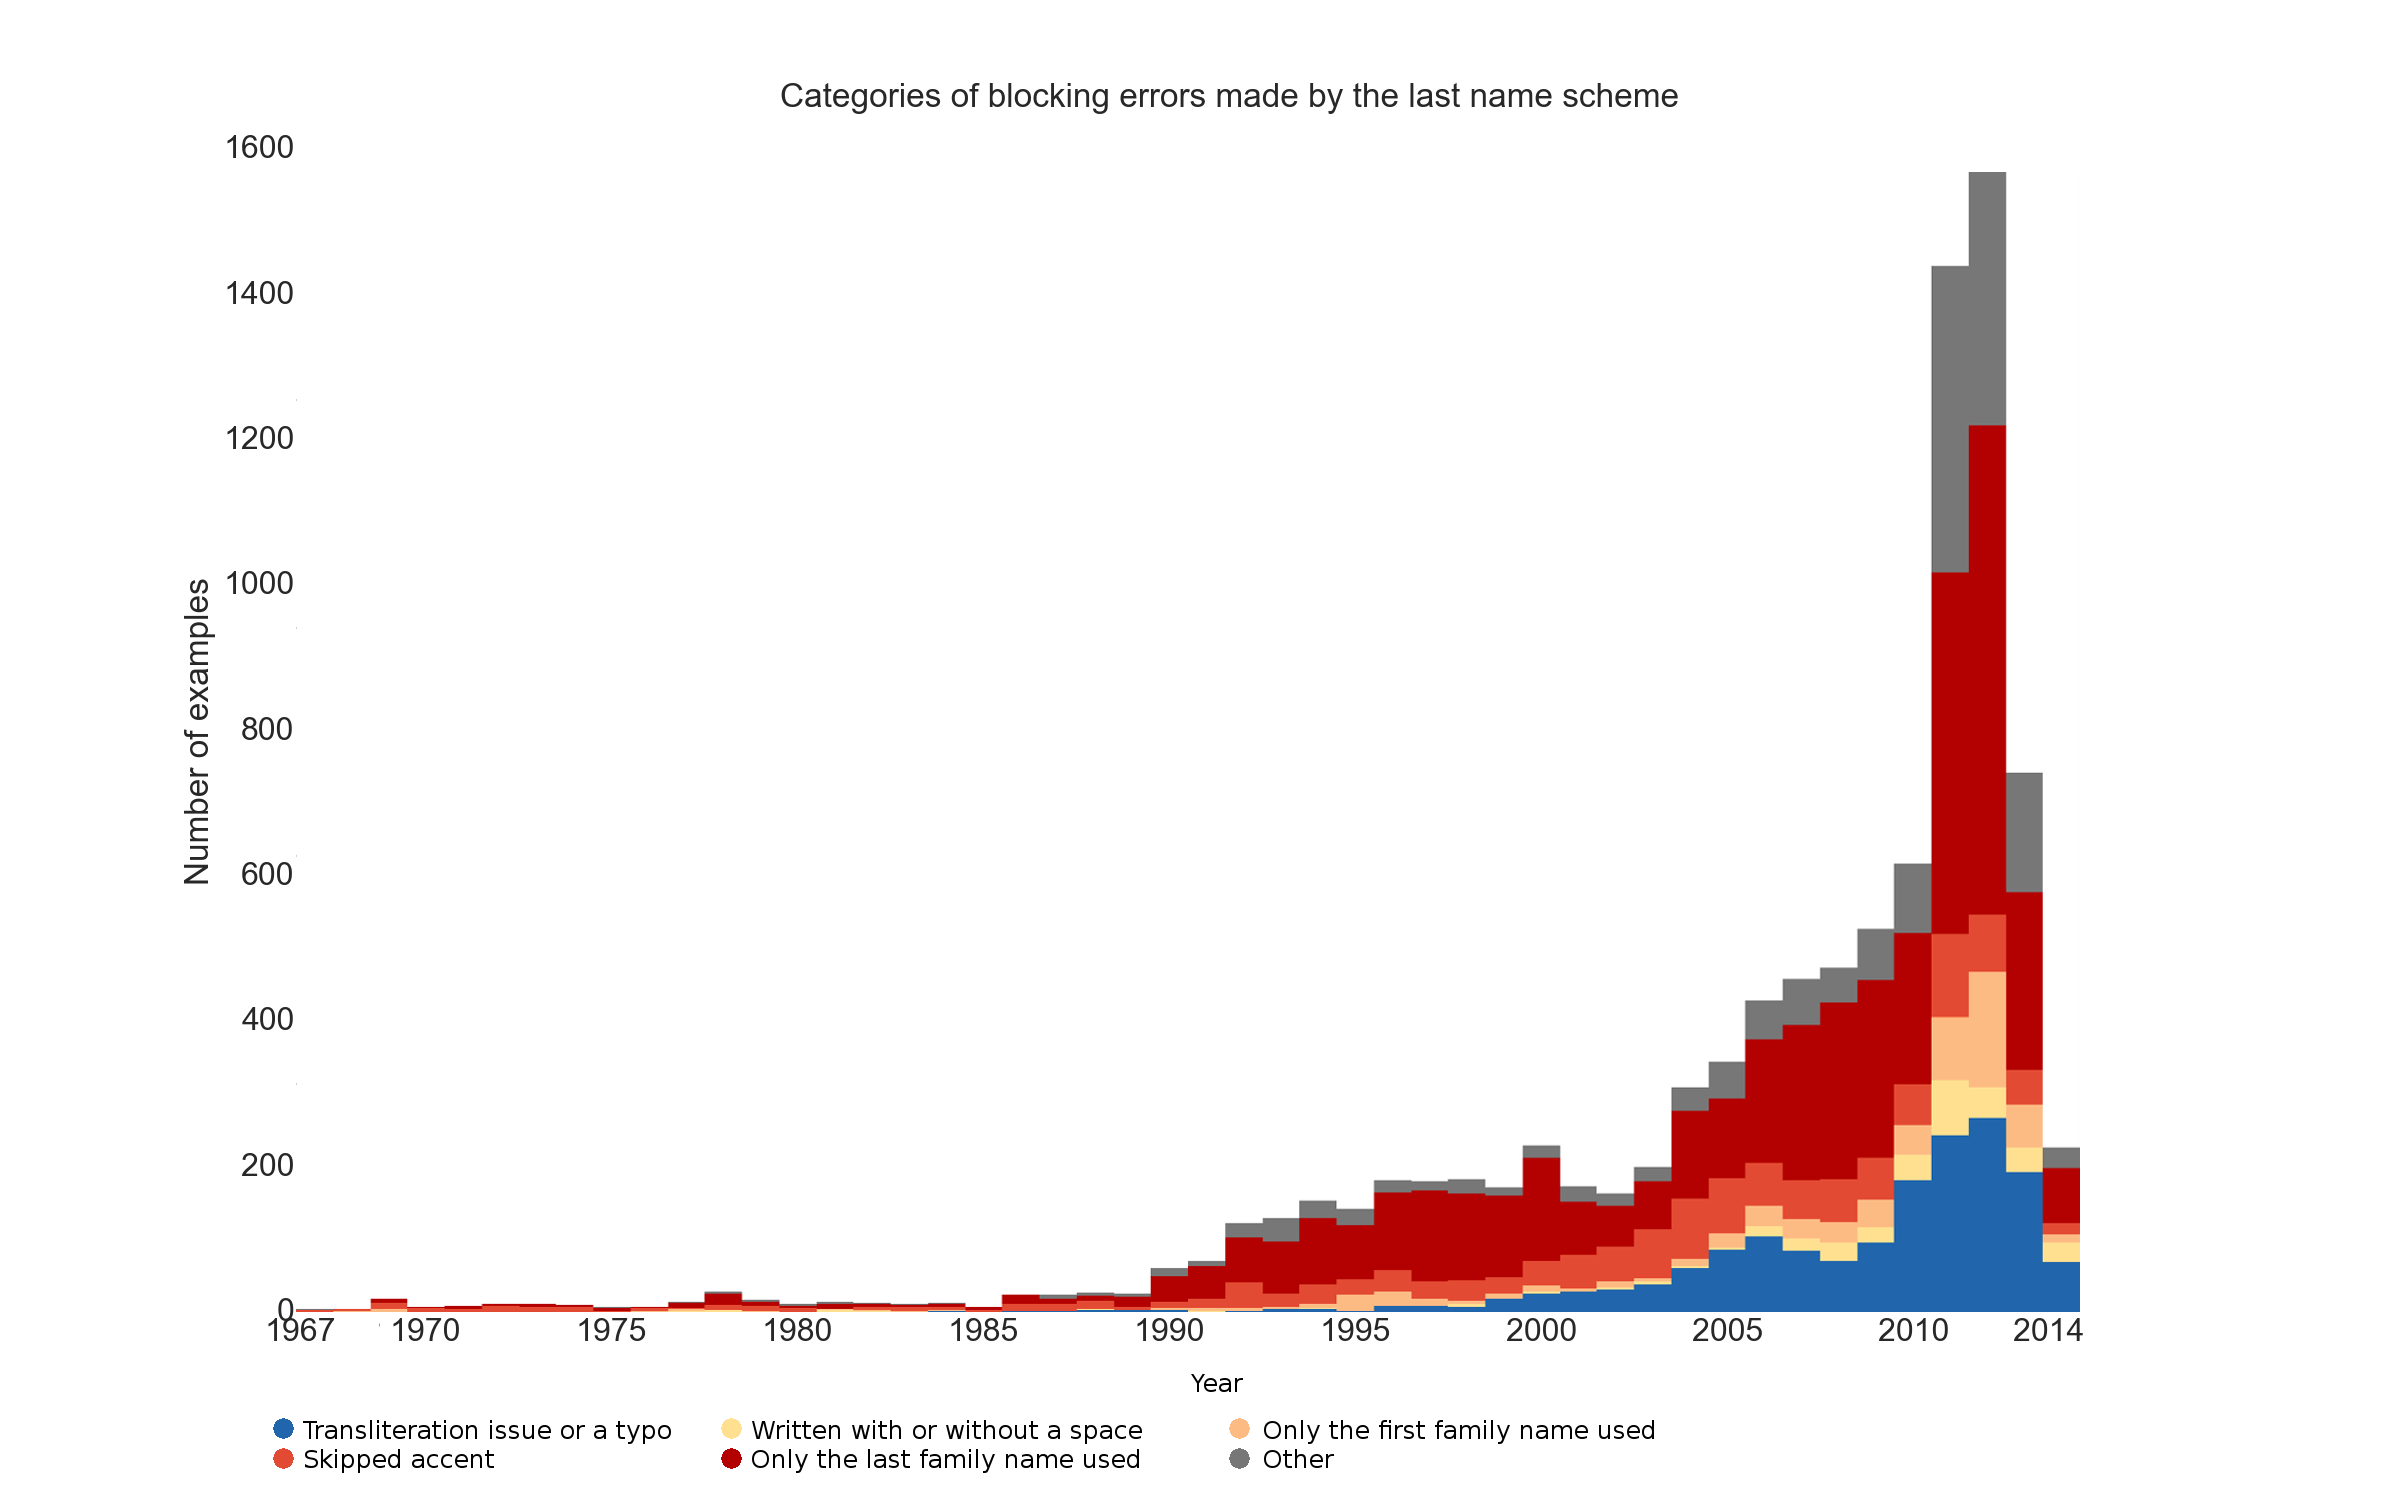
\includegraphics[width=\textwidth]{figures/blockerrors2}
\caption{Categories of blocking errors made by the last name scheme - number of
signatures with misinterpreted author's family name split over error categories.}
\label{fig:blockerrors2}
\end{sidewaysfigure}

\begin{sidewaysfigure}[p]
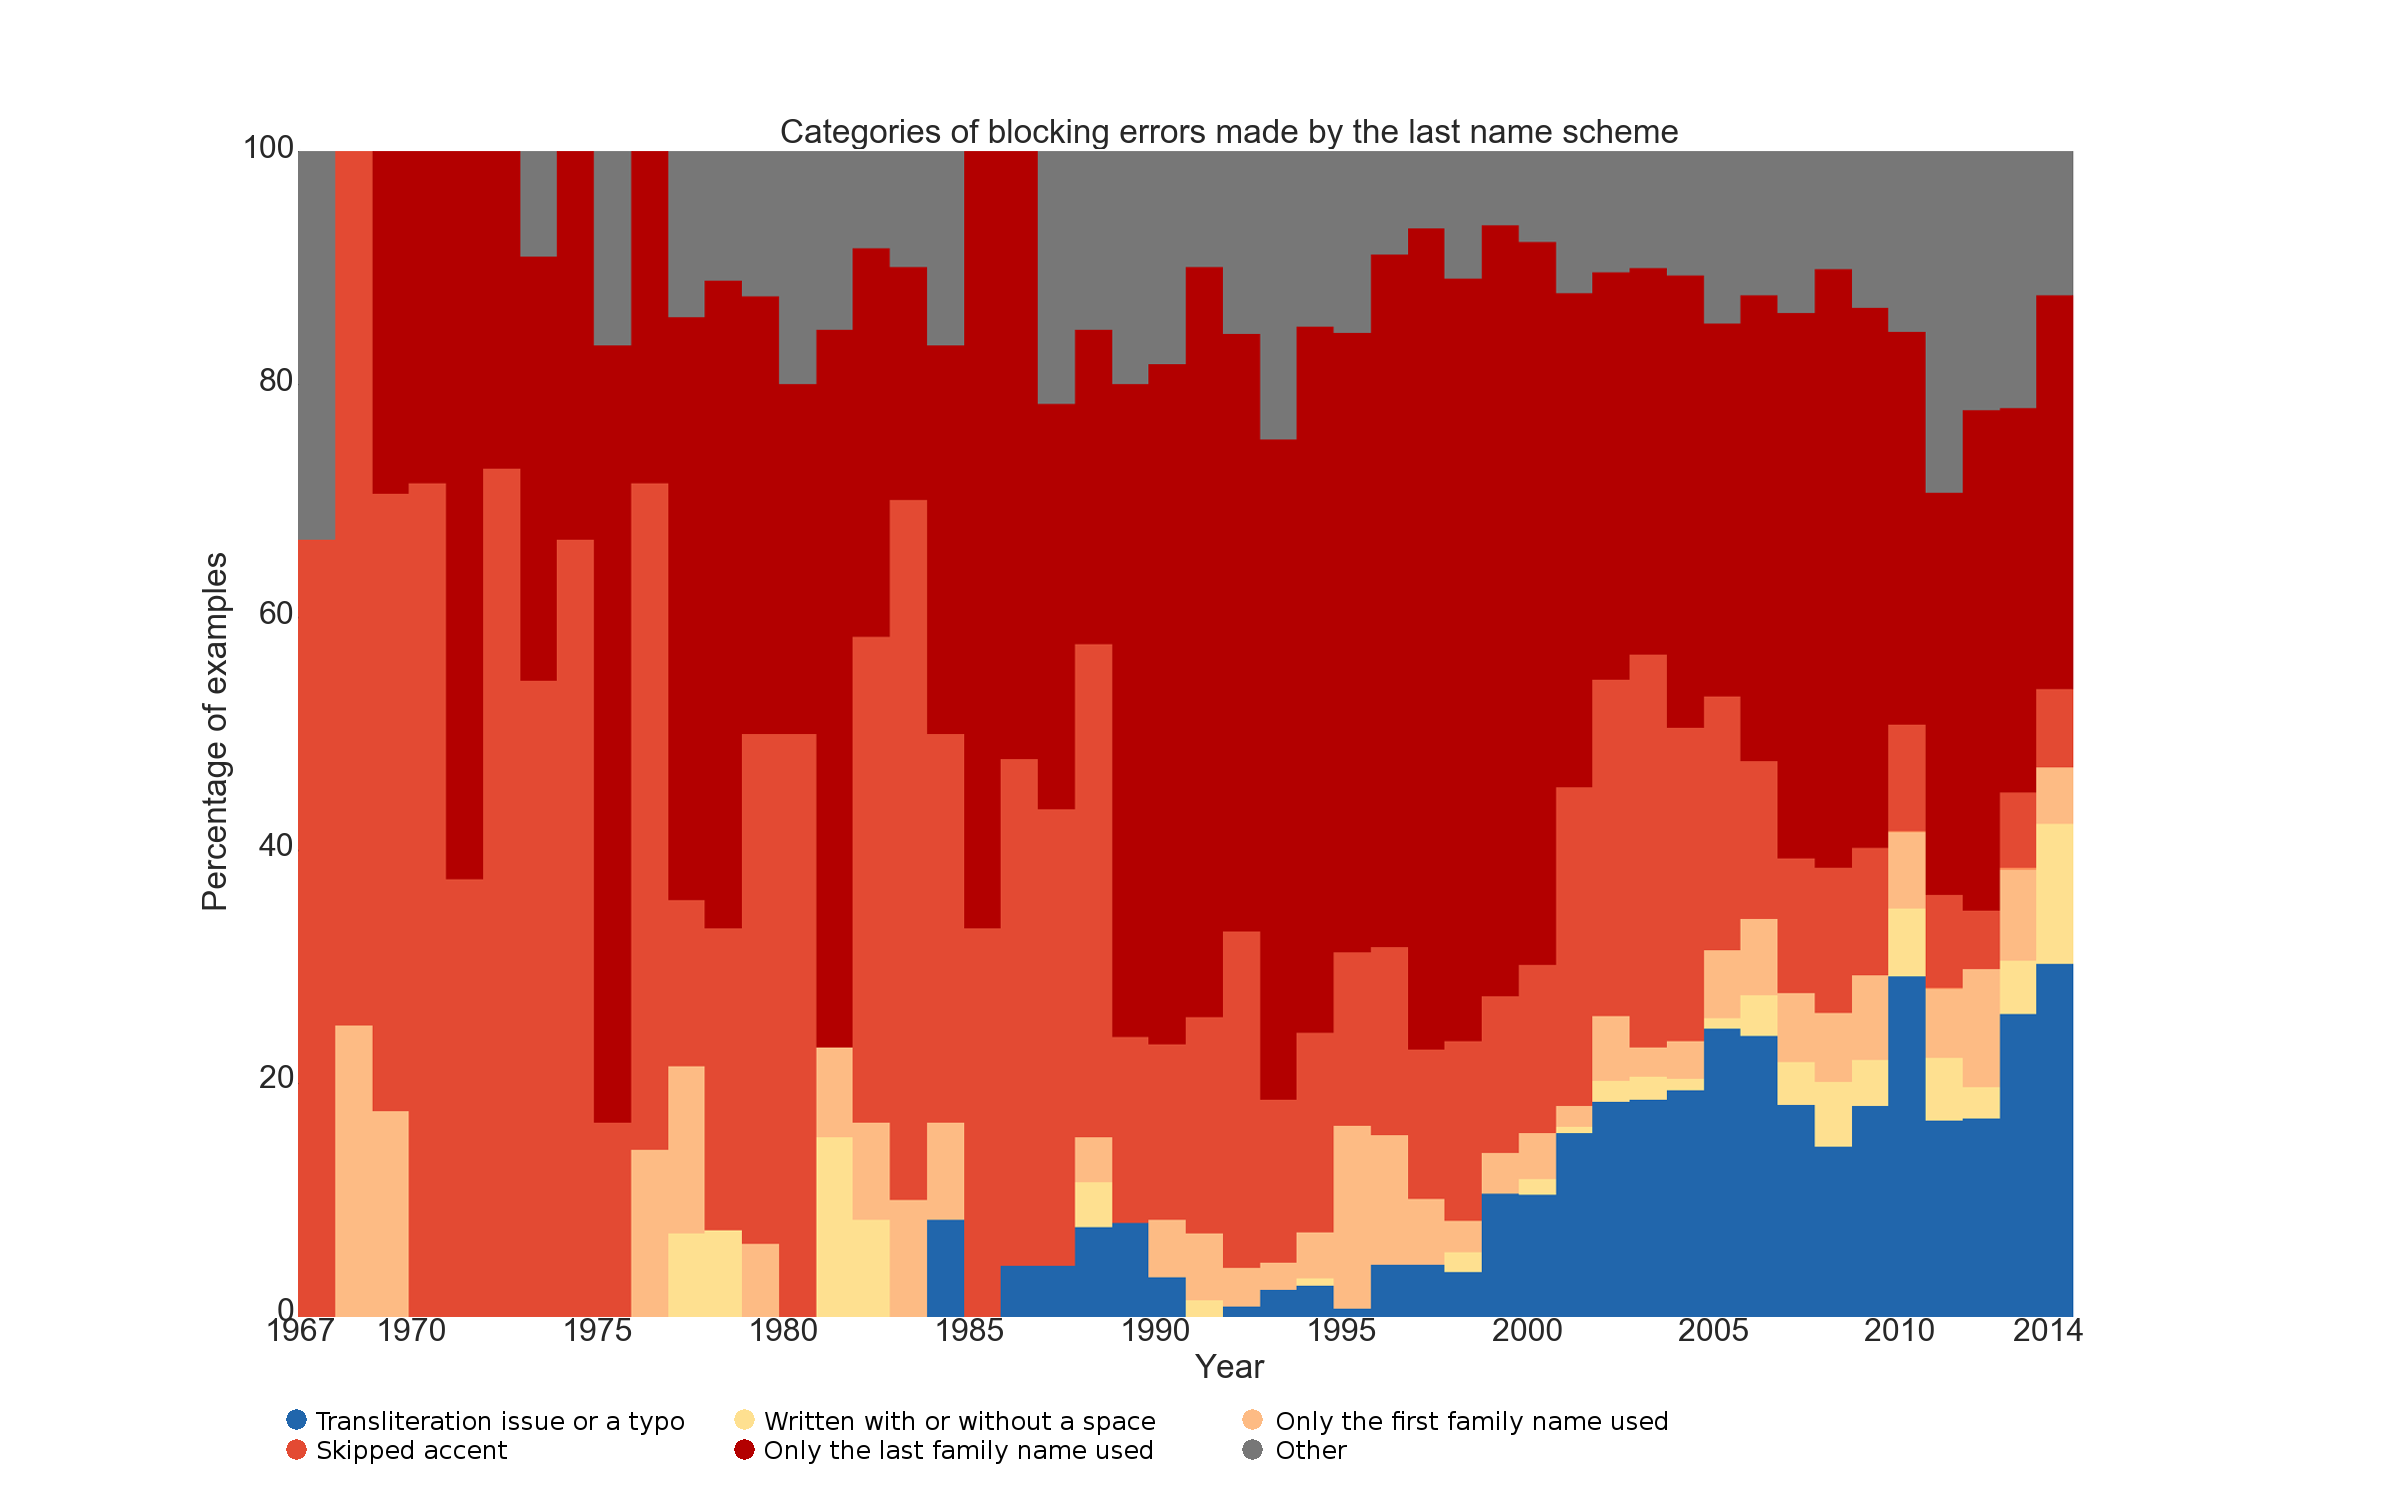
\includegraphics[width=\textwidth]{figures/blockerrors}
\caption{Categories of blocking errors made by the last name scheme - frequencies
of the error groups for each year.}
\label{fig:blockerrors}
\end{sidewaysfigure}

After the analysis were performed, a tailored solution could be implemented. Our approach
consists of few steps. Firstly the names are normalized. The normalization involves
the removal of diacritical marks, which appear inconsistently on the publications.
By doing so, we solve the \textit{Skipped accent} group. Moreover, some of the common
affixes were removed, as we observed some inconsistencies there. These cases were
classified as \textit{Only the first family name used} or \textit{Only the last family
name used} because the automatized retrieval solution treated every token as a new
family name. An example of this is a signature of \textit{van der Waals, J. D.}, which is
treated in the blocking phase as if it contained just the family name \textit{Waals} without
any prefixes. The hyphens are replaced by spaces. In the next steps of the algorithm
the affixes, hyphens and diacritical marks will be present on the names, as they
contain additional information.

After that, all the family names are processed by the phonetic algorithm. In case of
the \textit{Double Metaphone}, as this algorithm can output two possible phonetic
representation, always the first one is used. Here, the phonetic representations
of signatures that have only one family name already create the blocks. By doing so, the
category \textit{Transliteration issue or a typo} is effectively rooted out. 
The question is, how to handle signatures with multiple surnames (phonetic representations
of multiple surnames at this step). A simple strategy that reduces drastically the number 
of errors is to:

\begin{itemize}
    \item Check if the first family name of the author was used in the group of the
    phonetic representation of the last family name as the last given name on any of the
    signatures. If this condition is met, add this signature to this group.
    \item Otherwise check if the group of the phonetic representation of the last family
    name of the author exists. If this condition is met, add the signature to
    this group.
    \item Otherwise create a new group represented by the phonetic representation
    of the last family name.
\end{itemize}

This strategy effectively solves error categories
\textit{Only the first family name used} and \textit{Only the last family name used}.
The only category error that has not been fought is \textit{Other}. However, it seems
impossible to block together signatures with entirely different family names
maintaining the reduced sizes of blocks. Perhaps, some more sophisticated techniques can be
adopted. However, if too much focus is spend on this area, in order to solve the blocking
problem, a procedure that would imitate the whole disambiguation might be
developed.

In order to further reduce the sizes of the blocks, the computed blocks are split
over the first given name initials if they contain more than $1000$ signatures. This adds errors
only in situations where an author has multiple given names and the first one is not
always recorded. It happens rarely in the studied dataset.

\section{Linkage function learning}

\subsection{Pair sampling}\label{sec:sampling}

In the step of linkage function learning we want to train a classifier that will
correctly guess whether a pair of signatures belongs to one or two authors.
As our model is not expected to be perfect, we relax this constraint and require the model
to output the probability that two publications belong to the same author.

Before we dive into the description of the model and the features used, let us emphasize
that the choice of the pairs used as the training data might influence the quality of
our solution. Due to the size of the dataset we are working with, we have to select a
subset of all the available pairs. In this work, we will try and compare three different 
sampling techniques.

As this issue has not been brought up in the previous works, we assume that when the
disambiguation datasets were large enough to require sampling, the choice  of pairs
was fully random. This is the first technique used in our comparison. It will
be called \textit{Non-blocked, uniform}.

As our algorithm performs the blocking step before the model is learned, it is possible
to enhance the naive sampling. If two signatures belong to different blocks, it seems
counterintuitive to add such a pair to the training data, as the algorithm has already
decided that these signatures belong to different authors. Thus, we propose another
approach to sampling. The \textit{Blocked, uniform} technique samples, with replacement,
a block, and then, without replacement, a signature from this block. See Algorithm
\ref{blocked}. We believe that this technique will help pick the 
pairs of signatures that are hard to distinguish - the pairs that belong to two authors 
and belong to the same block.

However, we noticed that this technique tends not to choose often the pairs belonging to
different authors. The vast majority of pairs belonging to the same block belong to the
same author - the names are usually unique \citep{lange2011frequency}. We came up with
another approach where we divide the pairs into four categories:

\begin{itemize}
\item{Same names, same authors}
\item{Different names, same authors}
\item{Same names, different authors}
\item{Different names, different authors}
\end{itemize}

Then, for each category, our algorithm samples the same number of pairs, in the same way
the pairs in \textit{Blocked, uniform} were chosen. As many of the previous works relied
on the name comparison \citep{Ferreira:survey}, we believe that this technique will
further emphasize the tough examples and guide the model in the right direction. We
will call this improved technique \textit{Blocked, balanced}.


\begin{algorithm}[H]
    \caption{Blocked sampling}
    \label{blocked}
    \begin{algorithmic}[1] % The number tells where the line numbering should start
        \Procedure{Blocked}{$blocks, sample\_size$} \Comment{blocks are sets of signatures}
            \State $pairs\gets \emptyset$
        	\While{$sample\_size\not=0$}
            	\State $block\gets sample(blocks)$
            	\If{$block$ contains a pair that has not been chosen yet}
                \State $new\_pair\gets sample(block.pairs() - pairs)$
                \State \Comment block.pairs() returns the set of possible pairs from the block
                \State $pairs.add(new\_pair)$
                \State $sample\_size\gets sample\_size - 1$
                \Else
                \State continue
            	\EndIf
            \EndWhile\label{euclidendwhile}
            \State \textbf{return} $pairs$
        \EndProcedure
    \end{algorithmic}
\end{algorithm}

\subsection{Features}

The basic version of the model used in this work is based on 22 features. 15 of them are
introduced arbitrarily and 7 of them are prelearned ethnicity features. Let us start with
the description of the former ones:

% TO DO n-grams
\begin{itemize}
\item{\textit{Year difference} - the absolute difference between the years of publication
of the papers with the compared signatures.}
\item{\textit{Given name initial} - a boolean variable equal to 1 if the first given
names initials on the signatures are the same and 0 otherwise.}
\item{\textit{First given name} - the Jaro-Winkler distance \citep{winkler} of the first
given names from the signatures.}
\item{\textit{Second given name} - the Jaro-Winkler distance \citep{winkler} of the second
given names from the signatures. An empty name is used when the signature does not
contain a second given name.}
\item{6 features computed as cosine similarities of the TF-IDF vectors of the
metadata fields from the papers with the compared signatures. The fields used were
the categorical text fields, and TF-IDF vectors were computed on the categories. The
fields creating the features are:

\begin{itemize}
\item{Abstract}
\item{Keywords}
\item{Collaborations}
\item{References}
\item{Subject}
\item{Co-authors - this field was treated in a special way. As some of the papers
from the field of HEP are written by large collaborations, they have up to
thousand of authors. The TF-IDF vectors computed on all the tokens
coming from all these author would be very noisy and would not add meaningful
information. We improve it by taking
only the ten closest co-authors from the lexicographically sorted list.
This way the collaboration paper do not influence heavily the model.
Fortunately, Inspire stores the list of authors of the papers sorted in this way,
so there is no additional computational cost.}
\end{itemize}}

\item{5 features computed as cosine similarities of the TF-IDF vectors of the
(2-4)-grams of the metadata fields from the papers with the compared signatures.
The fields used were the descriptive text fields, and the n-grams were
computed on the whole fields. The fields creating the features are:

\begin{itemize}
\item{Full name}
\item{Given names}
\item{Affiliation}
\item{Title}
\item{Journal}
\end{itemize}}

\end{itemize}

\subsection{Ethnicity features}

As suggested by Chin et al. \citep{chin14a} because of different naming
conventions, it is beneficial to consider authors of different ethnicities
separately. The original work only tailored the solution to the case of Chinese
vs non-Chinese authors. We extend this technique and propose a model that represents the 
ethnicity as a vector in $\mathbb{R}^7$ where the dimensions correspond to the standard
classification of the ethnicities used in US Censuses\footnote{\href{https://en.wikipedia.org/wiki/Race\_and\_ethnicity\_in\_the\_United\_States\_Census\#Census\_2000}{https://en.wikipedia.org/wiki/Race\_and\_ethnicity\_in\_the\_United\_States\_Census\#Census\_2000}}. These are called:

\begin{itemize}
\item{White}
\item{Black}
\item{American Indian or Alaska Native}
\item{Chinese}
\item{Japanese}
\item{Other Asian or Pacific Islander}
\item{Others}
\end{itemize}

In order to model the ethnicity on the base of author's name, we trained a
SVM model with a linear kernel in one-vs-all approach. The input consisted of the TF-IDF
vectors of (1,5) n-grams build over the names taken from the US Census dataset provided by 
the Integrated Public Use Microdata Series (IPUMS). This dataset is a mapping from a name
to person's ethnicity. Following the licensing agreement of the IPUMS data, we are not
allowed to distribute this dataset (it is not available in the open-source
implementation).

The model, for each ethnicity, predicts the probability that a given name belongs
to a person having this ethnicity's background. Having such model, we create an
additional feature for each ethnicity. This feature is the product of probabilities
output by the model for names from both signatures from the pair.

\section{Clustering}

Having created a model that predicts well whether two signatures belong to the same
author or not, we have to encapsulate this knowledge in order to create disjoint
clusters. To further explain why the clustering step is necessary let us consider an
example where three signatures are disambiguated. The linkage function we created
tells us that with high probability two out of the three pairs are written by the same
author, while the remaining one probably belongs to two authors. In this case, it
is hard to say what should be the final solution. Instead of building a heuristic
that will clean this graph and create connected components, we should try few
different clustering approaches and benchmark them.

As disambiguation data is noisy and we do not have the knowledge about the true
number of authors in the whole system, we decided to try semi-supervised approach
in hierarchical clustering. We compare three different approaches:

\begin{itemize}
\item{\textit{No cut} - an approach where the linkage function is not required.
We treat the result of the blocking step as the result of the whole algorithm.}
\item{\textit{Global cut} - a semi-supervised approach where the blocks are split
into clusters using a global threshold. The clusters are disjoint if the distance
(in terms of the used clustering metric) between them is larger than the threshold.
In order to choose the threshold all the possible cuts are evaluated on the training
subset of all signatures, and the cut that maximizes the value of the evaluation
metric is chosen.}
\item{\textit{Block cut} - a semi-supervised approach where the blocks are split
into clusters using a local threshold. The clusters are disjoint if the distance
(in terms of the used clustering metric) between them is larger than the threshold.
In order to choose threshold all the possible cuts are evaluated on the training
subset of signatures from a block, and the cut that maximizes the value of the evaluation
metric is chosen for this block. This clustering technique chooses independently
a threshold for each block. In case where there are no available labeled signatures
in a block, a single cluster is created.}
\end{itemize}

\begin{figure}[th!]
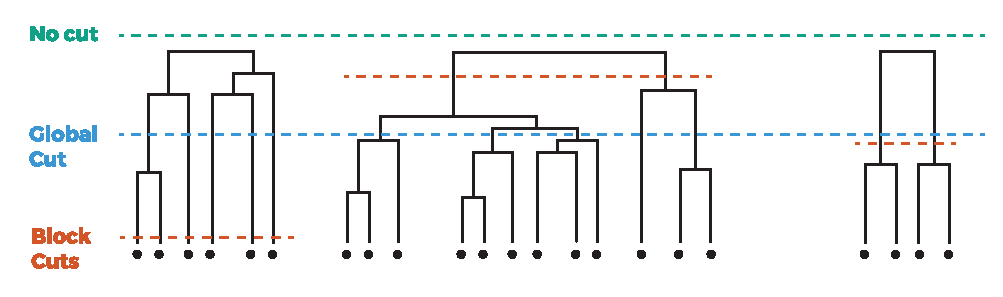
\includegraphics[width=\textwidth]{figures/fig-cuts}
\caption{Illustration of the thresholding techniques proposed. The \textit{No cut}
technique assumes the blocks are the desired clusters. The \textit{Global cut}
makes the cut that maximizes the score on all the training examples. The
\textit{Block cut} for each block makes the cut that maximizes the score
on the training samples from the given block.}
\label{fig:cuts}
\end{figure}


By using the block cut we can tailor our clustering to each block, treating
each of the blocks as an entirely separate disambiguation problem.

The resulting clusters are the result of the whole algorithm.


\chapter{Cluster matching}\label{sec:clustermatch}
The clusters computed by our algorithm can not be used in the digital library as long as
they are not matched with the clusters that existed before. The author profiles
available in Inspire contain additional information and some of them are assigned
to the users of the portal. Thus, it is not a viable option to drop the profiles
after the disambiguation and replace them with empty profiles created from the new
clusters. It is important to create a relationship between the new and the existing clusters.
We can reduce the issue to the \textit{assignment problem} if we assign one (and not
more) unique new cluster to each existing cluster.

Firstly, we will say why a clever solution is required. Let us simplify the
disambiguation problem and present it as a 2D clustering problem. The example
shown below on Figure \ref{fig:matching1} shows this simplified disambiguation performed
after an arrival of new signatures.
\\
\\
\\
\\
\\

\begin{figure}[H]
\center{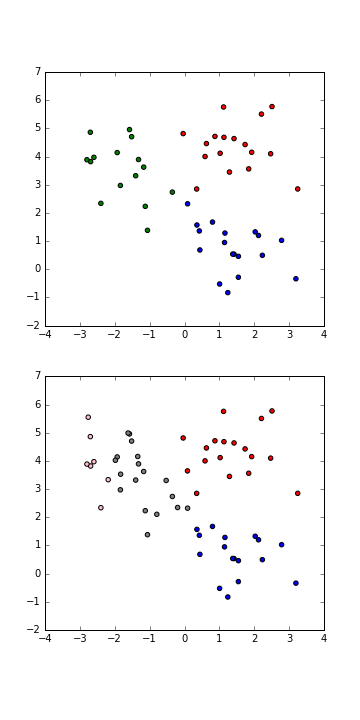
\includegraphics[height=1.4\textwidth]{figures/oldnew}}
\caption{Difference between new and existing clusters. On the top, the old disambiguation
is pictured. Each point represents a signature in this 2-dimensional space.
There are 3 clusters (red, blue and green). After adding few
new signatures and performing the disambiguation, the result consists of 4 clusters
(red, blue, pink and gray).}
\label{fig:matching1}
\end{figure}

The interesting thing is, that there is no clear answer if the pink or the gray
cluster is the new one. In the assignment problem, one of the
inputs is the cost of relationship in any possible pair. We can define the cost of
assigning a new cluster $A$ to an existing cluster $B$ taking into account few factors,
for example:

\begin{itemize}
\item{Number of signatures shared by $A$ and $B$}
\item{Number of signatures that are contained within $A \cup B$ but not within
$A \cap B$}
\item{Number of signatures from $A$ that were claimed (see Section \ref{inspire}) and
are contained within $B$}
\item{Number of signatures from $A$ that were claimed and
are not contained within $B$}
\end{itemize}

If we have such a function defined, we can solve the assignment problem. A standard
polynomial solution is Hungarian Algorithm \citep{kuhn}. The optimal implementation runs in
$\mathcal{O}(n^3)$ time \citep{tomizawa}. Thus, it can not be used in our solution,
as it would be too slow. Instead, we propose to express the assignment problem
as a linear programming problem.

\begin{mydef}
Assignment problem in terms of a relaxed linear program is:
\begin{equation*}
\begin{array}{ll@{}ll}
\text{minimize}  & \ \ \displaystyle\sum\limits_{j=0}^{K_{b}-1} &\displaystyle\sum\limits_{i=0}^{K_{a} + K_{b} - 1} c_{ij}x_{ij} &\\
\text{subject to}& \ \ \displaystyle\sum\limits_{j=0}^{K_{b}-1}   &x_{ij} \leq 1,  &i=0 ,..., K_{a} + K_{b} - 1\\
                 & \displaystyle\sum\limits_{i=0}^{K_{a} + K_{b} - 1}                                               &x_{ij} = 1, &j=0 ,..., K_{b}\\
                 \\
                 & x_{ij} \geq 0 &
\end{array}
\end{equation*}
where \\
$K_{a}$ - number of existing clusters \\
$K_{b}$ - number of new clusters \\
$c_{ij}$ - cost of linking an existing cluster $i$ with a new cluster $j$. Note that there are
additional $K_{a}$ empty new clusters, as all of the existing clusters need to be matched (so
that the profile data is not lost). 
$x_{ij}$ - edges
\end{mydef}

The explanation for this linear program is:
\begin{itemize}
\item{The first constraint limits the number of possible outgoing edges from an existing cluster
to 0 or 1}
\item{The second constraint limits the number of possible outgoing edges from a new cluster
to 1}
\item{The third term relaxes the problem}
\end{itemize}

Due to the statement of the problem, the solution yielded by the simplex algorithm is
guaranteed to be integer (the constraint matrix is unimodular). With the sophisticated
algorithm like Simplex \citep{simplex} the algorithm should run in reasonable time.

The design of the cost function is not a part of this thesis, and thus no results for this
part will be provided.


\part{Implementation}

\chapter{Library}

The solution proposed in this work can be easily reused using the open-source
implementation available on
Github\footnote{\href{https://github.com/inspirehep/beard}{https://github.com/inspirehep/beard}}
called Beard.
The solution was implemented in Python. The classifiers: SVM, CART, Random Forest,
Gradient Boosting and Linear Regression come from proven Scikit-learn library
\citep{scikitlearn}. The MLP used in this work was implemented using Keras
\citep{chollet2015}. The hierarchical
clustering comes from SciPy \citep{scipy}. The API of the Beard library follows
the Scikit-learn API and the best practices suggested by the authors of
Scikit-learn \citep{scikitlearnAPI}.

The implementation of the clustering is parallelized. This is done by computing
the dendograms of few blocks in the same time independently. The other time consuming
step is the linkage function learning. If the user of the library uses the random forest
algorithm, the parallelization comes from the Scikit-learn library. In the case
of the gradient boosting, the parallelization will be available when it will be
integrated into Scikit-learn\footnote{\href{https://github.com/scikit-learn/scikit-learn/issues/3628}{https://github.com/scikit-learn/scikit-learn/issues/3628}}. However,
if better performance for gradient boosting is needed, we suggest using XGBoost library,
which is easy to plug in to Beard.

It is important to note that our implementation of author disambiguation make it possible
to run the algorithm incrementally. If the signatures were disambiguated in the past,
only the blocks with new signatures have to be disambiguated. Moreover, the linkage function
learned during the previous disambiguation can be reused.

Beard is available on the standard Python package manager: PyPI.


\chapter{Project environment}

The algorithm that is the contribution of this thesis was developed for the
\textit{Inspire} project. \textit{Inspire} is a digital library developed by \textit{CERN}
based on \textit{Invenio} framework for rapid creation of digital libraries. In this chapter
we will introduce in detail the reader into the environment of the project.

\section{CERN}
\textit{CERN} (\textit{Organisation Europ\'eenne pour la Recherche
Nucl\'eaire}\footnote{Yes, we know that it should be abbreviated as OERN. The popular,
official abbreviation comes from the first, historical name of the
organization - \textit{Conseil Europ\'een pour la Recherche Nucl\'eaire} }) is a research
center focusing on the subject of high energy physics physics. Its recognizability among
people who are not related to scientific research comes from the fact that as of 2017 it
possesses the biggest particle accelerator in the world - \textit{LHC}. \textit{CERN} is
located on the border between France and Switzerland, west of Geneva.

Some of the big inventions created at \textit{CERN} transcend physics. In 1989 Timothy
Berners-Lee created a communication protocol which led later to the creation of
\textit{HTTP}. In 1990 he created the first web browser - \textit{WorldWideWeb} - and the
first web server.

The history of \textit{CERN} begins in February of 1952 when representatives of 12 European
countries signed a creation document. Since then, the organization has been placing particular 
emphasis on international cooperation and knowledge exchange. Nowadays, there are 22 member 
countries, and employees \citep{cps} from various parts of the world contribute to the
scientific advance. In the context of software, \textit{CERN} works on spreading the idea of 
developing only open source solutions and releasing open data.

\section{Invenio}
\textit{Invenio} is one of many open source projects developed at \textit{CERN} that were
created in order to provide easier access to science. It is a framework that supports rapid
building of digital libraries and document repositories. It aims at efficient handling of
large document databases. It has been successfully used by services such as: \textit{Inspire},
\textit{CERN Document Server}, \textit{Zenodo}, \textit{JINR Document Server}, and many others 
\footnote{\href{http://roar.eprints.org/view/software/cdsware.html}
{http://roar.eprints.org/view/software/cdsware.html}}.

\section{Inspire}\label{inspire}
\textit{Inspire} is a digital library that succeeded the main literature database for high energy physics called \textit{Stanford Physics Information Retrieval System}. \textit{Inspire} is build on top of \textit{Invenio} framework for the purpose of offering more interactivity to the users than the previous system. As of 2015, it offers few additional services than enhance work of high energy physics scientists. Few of them are listed below:

\begin{itemize}
\item HEPNames -A directory of researchers involved in the field of high energy physics
\item Institutions - A database containing information about institutes related to the field of high energy physics. As of 2015, this directory stores 11000 records.
\item Conferences - A database containing information about conferences held all around the world.
\item Jobs - A job board containing offers for scientists and staff members related to the field of high energy physics
\item Experiments - A database containing information about high energy physics experiments.
\item Journals - A database containing information about high energy physics journals.
\end{itemize}

This work focuses on the major feature of the \textit{HEPNames} service. Every researcher who wrote a publication contained within \textit{INSPIRE} has as well an \textit{author profile}. An \textit{author profile} is a summary of scientific career of the researcher. It is publicly available, thus it can be used as an indicator of research interests and quality of published work. Many institutions working in the field of high energy physics use author profiles while recruiting physicists in order to get an insight into the possible usefulness of a candidate. \\

\begin{figure}[!ht]
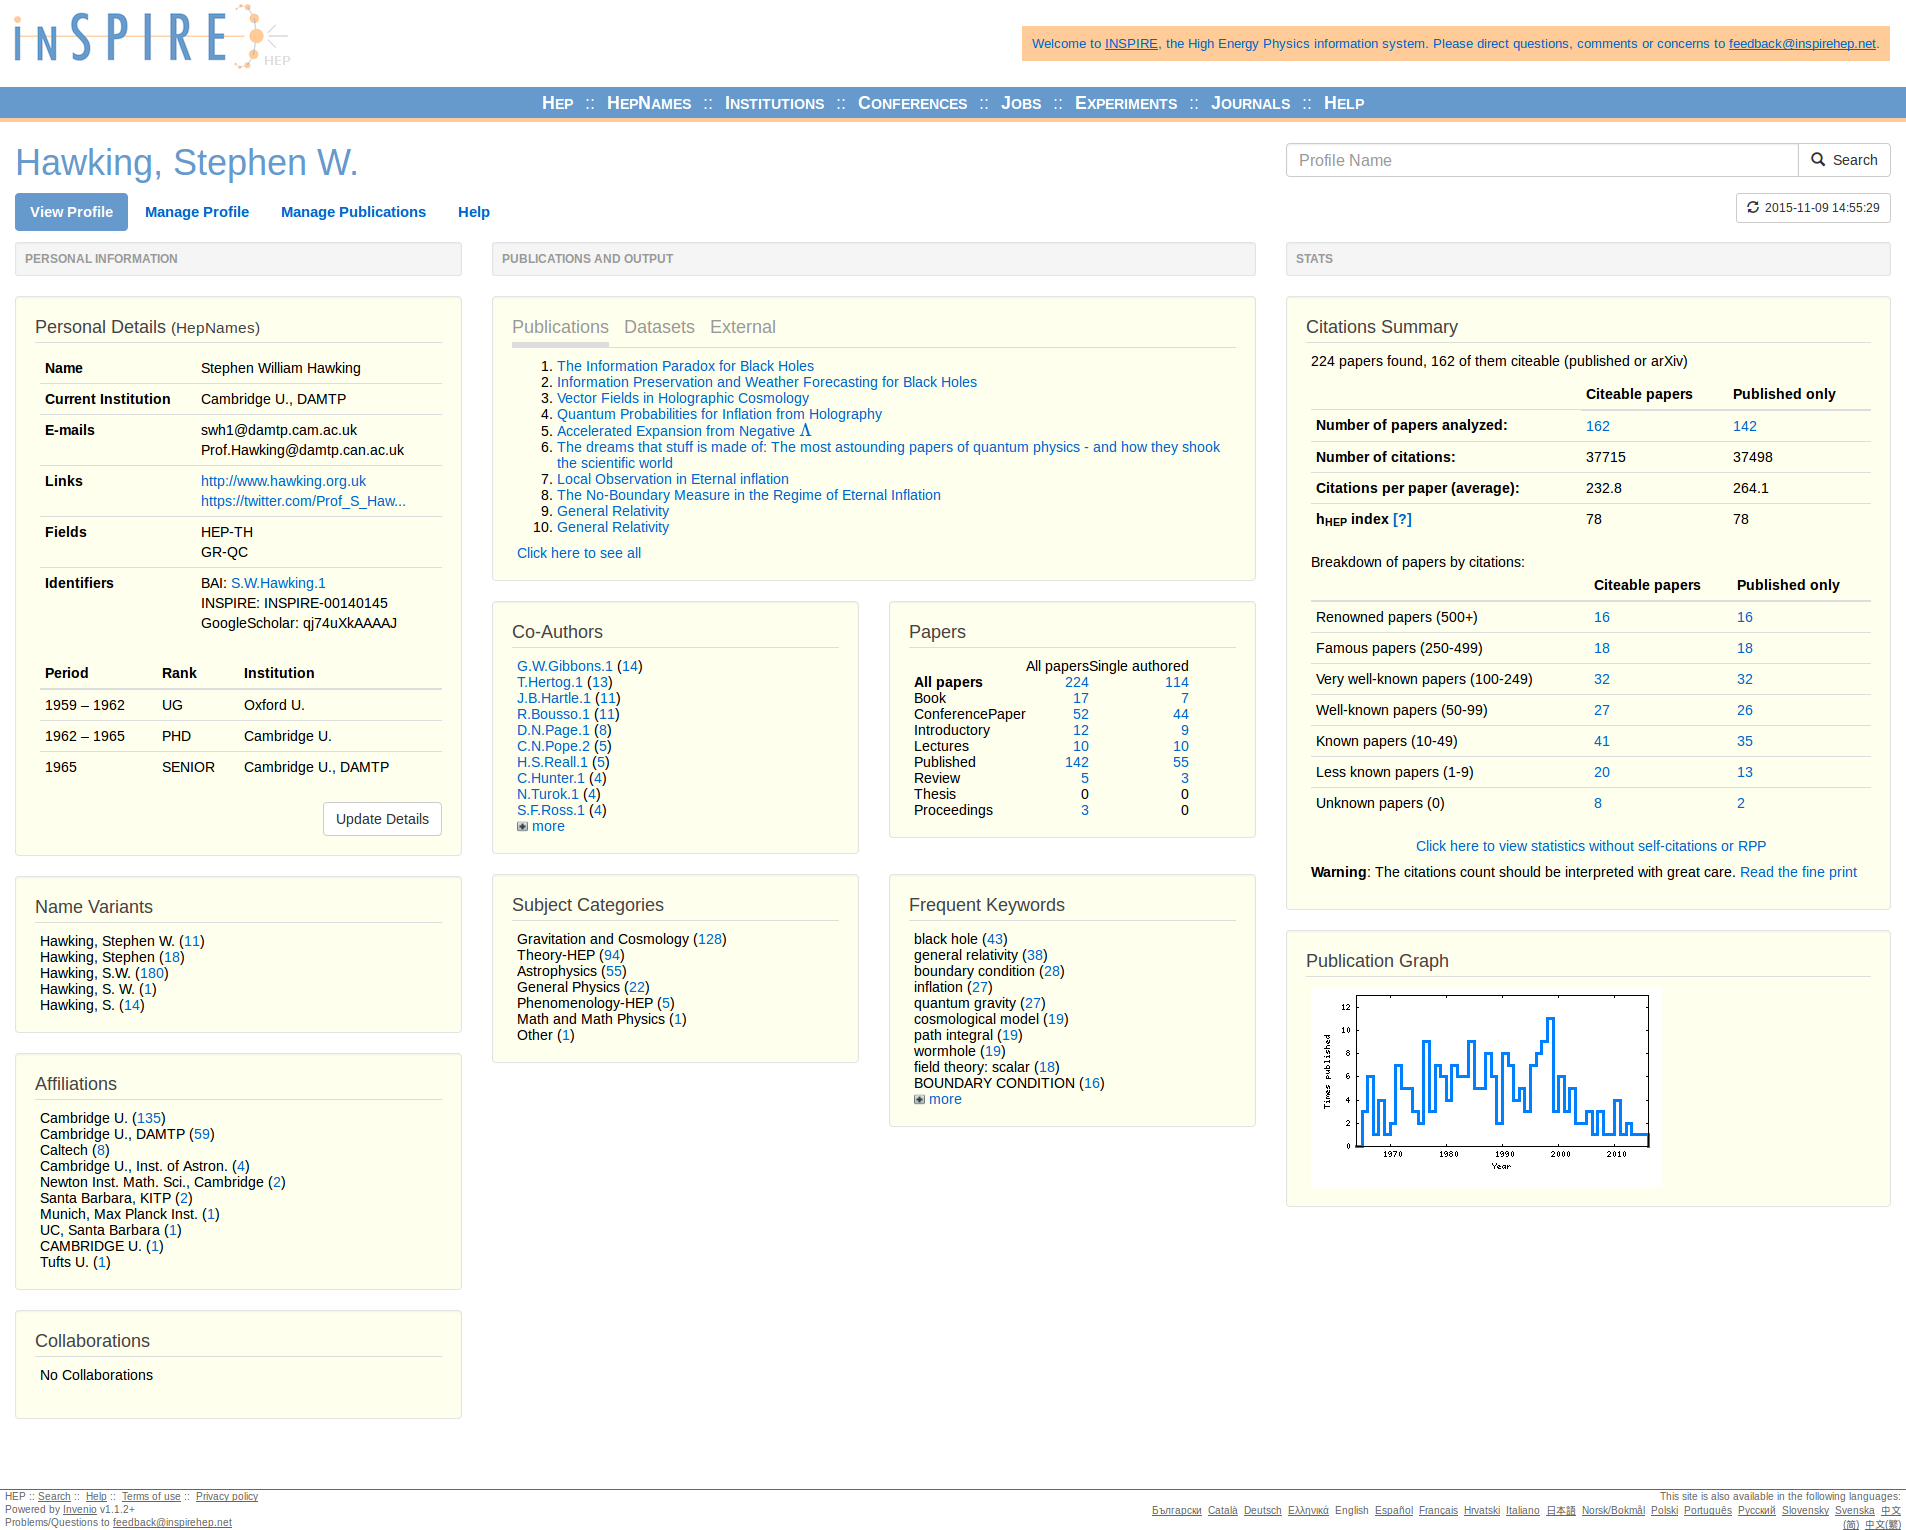
\includegraphics[width=\textwidth]{figures/profile}
\caption{The author profile of Stephen W. Hawking}
\label{fig:hawking}
\end{figure}


The scientific output on an author profile is represented as a handful of statistics. These statistics are computed using a relation between authors and signatures. Data is organized in boxes as presented on a figure Figure~\ref{fig:hawking}. Let's describe every box:

\begin{itemize}
\item \textbf{Personal Details} - Contains the most general information about the author - his name, history of affiliations, contact info, links to professional or personal websites, unique author identifiers (such as ORCID, Google Scholar ID, INSPIRE ID) and the list of fields the given person is working on. Note that this is the only box that uses mostly the data provided by users and it is only supported by the data coming from disambiguation algorithm. For example the history of institution does not extract the affiliations from the signatures.
\item \textbf{Name Variants} - Contains the list of the names as they appear on the signatures and number of appearances of each of them.
\item \textbf{Affiliations} - Contains the list of the affiliations of the author and number of appearances on signatures of each of them.
\item \textbf{Collaborations} - Contains the list of the collaborations of the author and number of appearances on signatures of each of them.
\item \textbf{Publications} - Contains the list of the 10 most recent publications the author wrote. This can include published papers, preprints and papers from \textit{ArXiv}.
\item \textbf{Datasets} - Contains the list of the 10 most recent datasets the author published. Note that the disambiguation algorithm treats datasets as publications.
\item \textbf{External} - Contains the list of the 10 most recent publications the author published that are not stored on \textit{INSPIRE}. As of 2015, \textit{INSPIRE} supported papers available on \textit{ORCID} and \textit{ArXiv}.
\item \textbf{Co-Authors} - Contains the list of co-authors and, for each of them, the number of publications written together.
\item \textbf{Subject Categories} - Contains the list of categories of the papers written by the author. For each of them the number of related papers is given.
\item \textbf{Papers} - Contains the number of papers and the number of papers in each of the following categories: \textit{Book}, \textit{Conference Paper}, \textit{Introductory}, \textit{Lecture}, \textit{Published}, \textit{Review}, \textit{Thesis}, \textit{Proceedings}. Additionally, the same statistics is available for the set of papers authored only by this author.
\item \textbf{Frequent Keywords} - Contains the list of keywords of the papers written by the author. For each of them the number of related papers is given.
\item \textbf{Citation Summary} - Contains crucial statistics for citations. Given are: number of citations, average number of citations per paper, h-index, and a categorization of papers by number of citations. The data is available also for the subset of published papers.
\item \textbf{Publication graph} - Contains a graph which shows how many papers the author wrote each year.
\end{itemize}

The service is popular among the researchers, as it offers a broad database of publications, 
up-to-date information and it allows the user to improve the data in the service. Every author
is entitled to report improvements in publications metadata. Moreover, the signatures can be 
assigned permanently to their authors by a \textit{claim}. 

Every \textit{claim} is recorded in the \textit{INSPIRE} database. A \textit{claim} can come
from the author itself, or 
any researcher who knows who wrote the publication. Thanks to this fact, \textit{Inspire} 
collected a very large manually curated signatures database that can be used as the training data 
in the algorithm 
we describe. It is important to note that the data stored in the INSPIRE database uses
MARC 21 format that has limited extensibility, effectively limiting the spectrum of the
metadata. Only some of the fields can be used as features in the algorithm we describe.
Further in this work we will use the word \textit{claimed} to describe a relation between a 
signature and an author in the ground truth dataset.


\section{Deployment}

As of 2016 Beard is fully integrated into Inspire providing accurate disambiguation
for this HEP digital library\footnote{\href{https://github.com/inspirehep/beard-server}{https://github.com/inspirehep/beard-server}}. The library runs a daemon that
periodically disambiguates blocks with new signatures.

\part{Experiments and results}


\chapter{Dataset}

The lack of a common benchmark that we mentioned while reviewing the related works
(see \myhy{sec:related}{Section 3.2}) is an issue for the author disambiguation
problem, as
the solutions proposed from various scientists can not be directly compared with
each other. In order to overcome this problem, we decided to publish the dataset
that we have been working with. All the signatures are labeled
and they come from \textit{Inspire} portal\footnote{The dataset is available on Github: \href{https://github.com/glouppe/paper-author-disambiguation/tree/master/data}{https://github.com/glouppe/paper-author-disambiguation/tree/master/data}}.

The dataset consists of the following files, all in JSON format \citep{EcmaScript}:

% 

\begin{itemize}
\item \textit{clusters.json} - dictionary of partially known clusters, in the form of:
\begin{lstlisting}
{cluster_id_1: [signature_id_1, ..., signature_id_N],
 cluster_id_2: [...], ... }
\end{lstlisting}
\item \textit{signatures.json} - dictionary of signature metadata, in the form of:
\begin{lstlisting}
{signature_id_1: {"author_name": "Doe, John", ...},
 signature_id_2: {...}, ...}
\end{lstlisting}
\item \textit{records.json} - dictionary of publication metadata, in the form of:
\begin{lstlisting}
{publication_id_1: {"title": "Lorem Ipsum", ...},
 publication_id_2: {...}, ...}
\end{lstlisting}
\end{itemize}

Additionally, in order to make our result completely reproducible, we published
the split of our dataset into 3 folds that were used in our cross validation
setup throughout all the experiments.

Our dataset consists of 1,201,763 signatures from 360,066 publications. These
signatures belong to 15,388 distinct authors who use 36,340 unique variants
of theirs names. The publications cover few decades starting from 1967 up to 2014.

On the next page we present three figures that describe the dataset. One can
notice that the publications come mainly from physics, mainly high energy physics
(HEP) and astrophysics (Figure \ref{fig:dat3}). It is important to note that
a paper can have no categories (i.e. this metadata is missing) and it can
have multiple categories.


\begin{figure}[!ht]
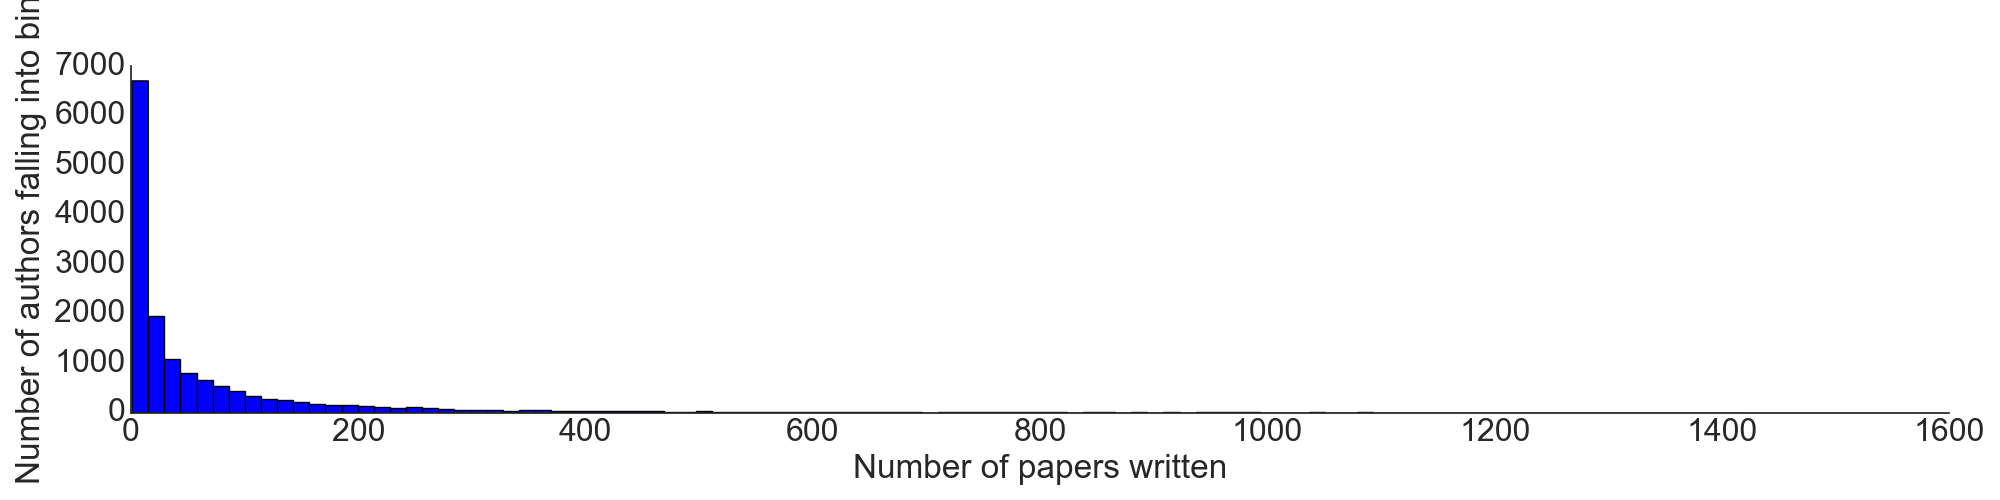
\includegraphics[width=\textwidth]{figures/counts}
\caption{Number of clusters of given size}
\label{fig:dat1}
\end{figure}


\begin{figure}[!ht]
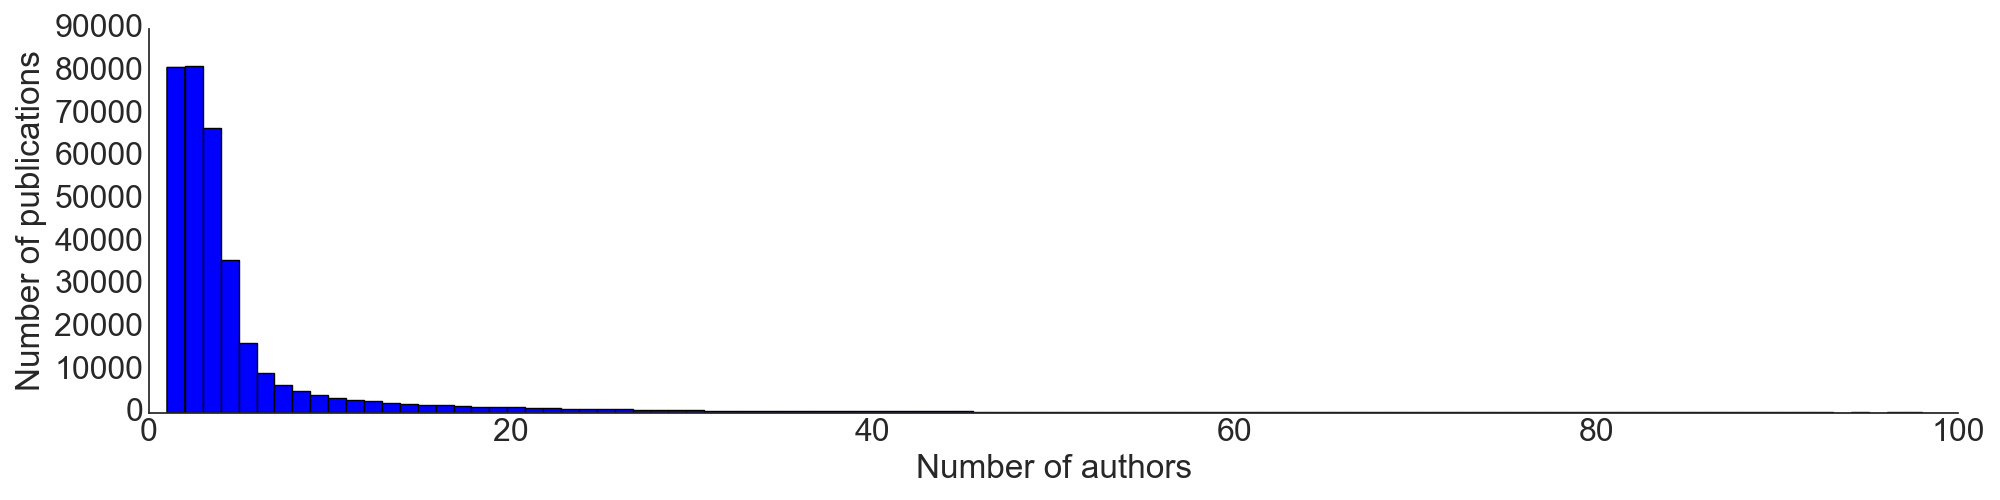
\includegraphics[width=\textwidth]{figures/counts2}
\caption{Number of publications written by a given number of authors.
Rare publications written by more than 100 authors (mostly collaborations) are not included.}
\label{fig:dat2}
\end{figure}


\begin{figure}[!ht]
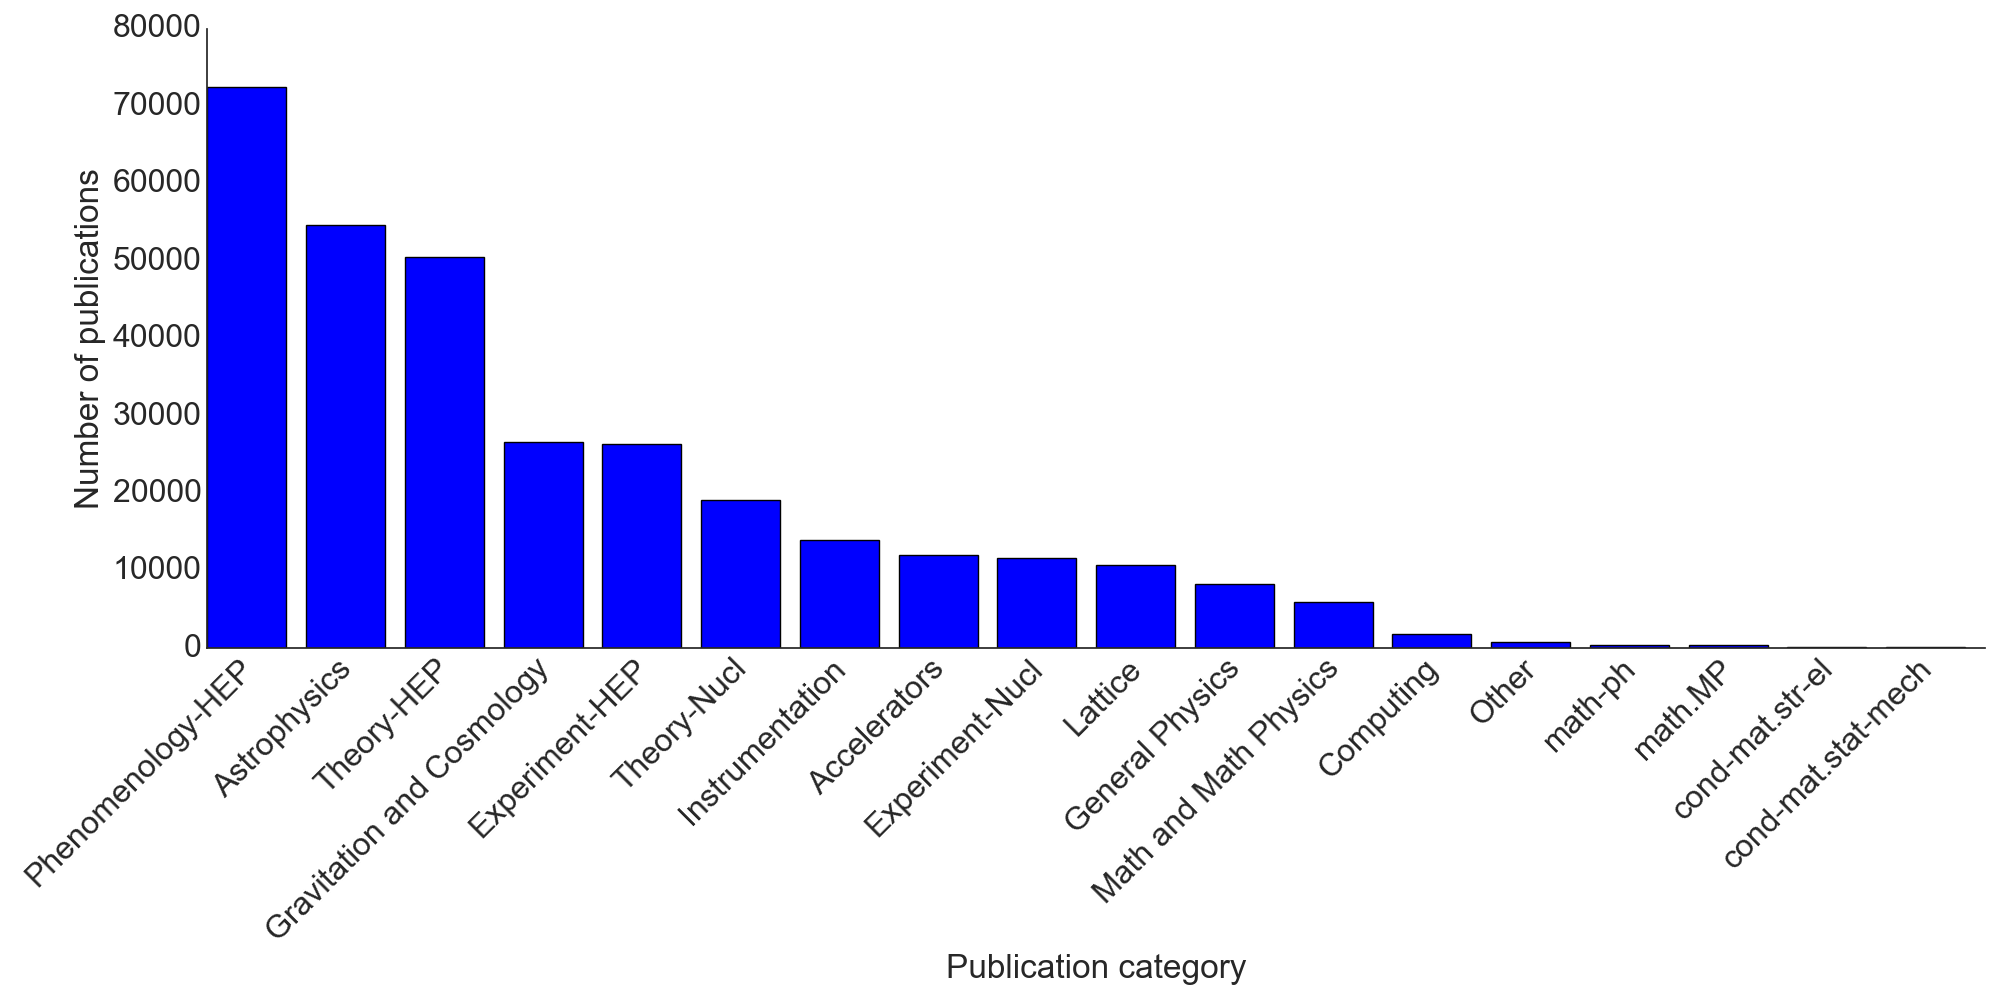
\includegraphics[width=\textwidth]{figures/topics}
\caption{Number of publication by category. Only the categories with at least
100 papers in the set are shown.}
\label{fig:dat3}
\end{figure}

Despite the efforts of the curators to keep
this data clean, we observed that a small percentage
of signatures is mislabeled. For example, due to the bugs in the code of
\textit{Inspire}, for a short period of time, when a user wanted to claim his
publication, and his name was not available in the metadata (i.e. one of the
signatures was missing from the metadata), the signature from another author
was used. It led to labels that were obviously wrong, as the signature of
a co-author was assigned to the user. It is possible to put more effort into
automatic discovery of erroneous signatures, which might led to a better
disambiguation.



\chapter{Testing environment}

The majority of the experiments requiring CPU were run on a machine with 32 GB RAM and a 16 core 
Intel Xeon processor. The machine was running on a Debian 7 operating system. Additionally,
some of the experiments requiring GPU were performed on another machine for linkage function step.
This machine was equipped with a GeForce GTX Titan Z graphic card.

The suggested pipeline using random forest and hierarchical clustering takes few hours to complete
on our dataset. Learning the linkage function on 1 million extracted
pairs took approximately 3 hours and clustering \~1,2 million signatures took approximately 3
hours 20 minutes. Other algorithm steps are computationally less demanding and they take at most
few minutes to complete.
The full clustering on the Inspire portal (9 million signatures after adding unlabeled data)
took around 23 hours.

\section{Evaluation}\label{sec:evaluation}

In order to compare different techniques, a proper evaluation metrics have to be defined.
The previous works on entity resolution used \textit{pairwise $F_{1}$ score}
and \textit{$B^{3}$ $F_{1}$ score}.

For the following definitions, let us denote:

\begin{itemize}
\item{${\cal S}$ - set of all signatures;}
\item{${\cal C}$ - set of predicted clusters;}
\item{$\widehat{\cal C}$ - set of ground-truth clusters;}
\item{$p(D)$ - set of all pairs of signatures from the same cluster in clusters $D$;}
\item{$c$ (resp. $\widehat{c}$) - predicted (resp. ground-truth) cluster that
given signature belongs to.}
\end{itemize}

\begin{mydef}
The pairwise $F_{1}$ score ($F_{pairwise}$) is defined as:
\begin{align}
F_\text{pairwise}({\cal C}, \widehat{\cal C}) &= \frac{2 P_\text{pairwise}({\cal C}, \widehat{\cal C}) R_\text{pairwise}({\cal C}, \widehat{\cal C})}{P_\text{pairwise}({\cal C}, \widehat{\cal C}) + R_\text{pairwise}({\cal C}, \widehat{\cal C})}\label{eq:test}
\end{align}
where $P_\text{pairwise}$ is pairwise precision and $R_\text{pairwise}$ is pairwise recall:
\begin{align}
P_\text{pairwise}({\cal C}, \widehat{\cal C}) &= \frac{|p({\cal C}) \cap p(\widehat{\cal C})|}{|p(\widehat{\cal C})|}\\
R_\text{pairwise}({\cal C}, \widehat{\cal C}) &= \frac{|p({\cal C}) \cap p(\widehat{\cal C})|}{|p({\cal C})|}
\end{align}


\end{mydef}
\begin{mydef}


The $B^{3}$ $F_{1}$ score ($F_{B^{3}}$) is defined as:

\begin{align}
F_\text{B3}({\cal C}, \widehat{\cal C}, {\cal S}) &= \frac{2 P_\text{B3}({\cal C}, \widehat{\cal C}, {\cal S}) R_\text{B3}({\cal C}, \widehat{\cal C}, {\cal S})}{P_\text{B3}({\cal C}, \widehat{\cal C}, {\cal S}) + P_\text{B3}({\cal C}, \widehat{\cal C}, {\cal S})}
\end{align}
where $P_{B^{3}}$ is pairwise precision and $R_{B^{3}}$ is pairwise recall:
\begin{align}
P_\text{B3}({\cal C}, \widehat{\cal C}, {\cal S}) &= \frac{1}{|{\cal S}|} \sum_{s \in {\cal S}} \frac{|c(s) \cap \widehat{c}(s)|}{|\widehat{c}(s)|} \\
R_\text{B3}({\cal C}, \widehat{\cal C}, {\cal S}) &= \frac{1}{|{\cal S}|} \sum_{s \in {\cal S}} \frac{|c(s) \cap \widehat{c}(s)|}{|c(s)|}
\end{align}

\end{mydef}

The pairwise $F_{1}$ score has its disadvantages. The biggest one is that focuses on large
clusters, diminishing the role of the small clusters in evaluation \citep{Barnes15}.
On the other hand, $B^{3}$ $F_{1}$ score is free from such shortcomings.
Moreover, it takes into account other factors, such as cluster homogeneity and cluster completeness
\citep{Amigo2009}. Thus, in the result summary, we will base our comments on the $B^{3}$ $F_{1}$ score.

In order to replicate the ratio of claimed vs. non-claimed signatures in Inspire, we
extract 13\% of all claimed signatures. From these signatures, we extract pairs as 
described in \myhy{sec:sampling}{Subsection 6.2.1}. The whole procedure is done three times
in order to form a 3-fold cross validation scheme. Throughout our result comparison we use
the same folds that are available at the dataset Github repository\footnote{\href{https://github.com/glouppe/paper-author-disambiguation/tree/master/data}{https://github.com/glouppe/paper-author-disambiguation/tree/master/data}}.

\section{Parameter setup}
For the linkage function learning step, the classifiers used there have to be parameterized.
Using standard grid search technique, we chose parameters for classifiers
by maximizing the $B^{3}$ $F_{1}$ score on one of the folds. The resulting choice is:

\begin{itemize}
\item{Random forest:}
\begin{itemize}
\item{Number of trees - 500}
\end{itemize}
\item{Gradient Boosting:}
\begin{itemize}
\item{Number of trees - 500}
\item{Maximum depth of a tree - 9}
\item{Maximum number of features used when looking for the best split - 10}
\item{Learning rate - 0.125}
\end{itemize}
\end{itemize}

The remaining parameters were default, as given in the original packages.

The neural network was constructed without the use of the grid search. Instead, two
architectures - one with three hidden layers of 22 neurons, and one with two hidden
layers of 22 neurons were examined. For both of them different values of dropout were tried.
After performing the experiments on a single fold, the network with two hidden layers and
dropout rate of 0.2 was selected.

\chapter{Results}

As most of the teams that have been working on author disambiguation did not release their
source code, we decided to create a solution that resembles the most interesting approaches.
Here, it will be called \textit{state-of-the-art}. The algorithm uses normalized names,
it blocks the signatures with the LNFI scheme, uses well parameterized gradient boosting and
UPGMA linkage hierarchical clustering with block cut. Note that state-of-the-art uses
sophisticated techniques than were not present in the related publications,
such as ethnicity features or block cuts.

Before we start with the comparison of techniques, we show the improvement achieved
(Table \ref{tab:15}). Although the improvement in score presented here is not exciting at the first
glance (the score improvement is measured in thousandths), even such difference can be crucial.
A $0.003$ improvement is $B^{3}$ $F_{1}$ score might correspond to the correction of thousands
of author profiles in the Inspire system. Thus, the improvement of $B^{3}$ $F_{1}$ score from
$0.9830$ to $0.9868$ is significant.


\begin{table}[H]
\caption{The general results. The best settings are the settings that achieved the
highest scores in this section.}
\centering
\begin{tabular}{|l|c c c | c c c|}
  \hline
                       & \multicolumn{3}{c|}{$\mathbf{B^{3}}$} & \multicolumn{3}{c|}{\textbf{Pairwise}}\\
  \textbf{Description} & $P$ & $R$ & $F$ & $P$ & $R$ & $F$ \\
  \hline
\hline
State-of-the-art & 0.9901 & 0.9760 & 0.9830   & 0.9948 & 0.9738 & 0.9842 \\
\hline
Combined best settings & 0.9888 & 0.9848 & \textbf{0.9868}  & 0.9951 & 0.9831 & \textbf{0.9890} \\
\hline
Best settings & & & & & & \\
without ethnicity features & 0.9862 & 0.9819 & 0.9841 & 0.9937 & 0.9815 & 0.9876 \\
  \hline
\end{tabular}
\label{tab:15}
\end{table}


\section{Blocking techniques comparison}
The first step of our algorithm is the blocking step. We will show two different comparisons
for evaluation of this algorithm. The first one consists of running the state-of-the art with
different blocking techniques. The results are shown in Table \ref{tab:10}.
As we can see, the proposed blocking algorithm, if used with
Double Metaphone or NYSIIS phonetic algorithm, outperforms LNFI strategy.
It is important to mention, that the advantage comes from the fact that the
new solution increases the recall. Intuitively, the recall drops when the
signatures belonging to the same author land in different clusters.
For example, a solution with a single cluster would have recall of $1$ and
precision of $0$. Using this knowledge we might observe that this improvement
in recall value comes from the fact that the new phonetic-based approach can
be interpreted as a procedure where the blocks from LNFI are merged.

Following this line of thought, we propose another comparison which shows us how
many errors are introduced by the blocking step.
Here, we compute the maximum possible recall after
the blocking step is performed. The computation is trivial. If we
evaluate the solution where the blocks are the clusters, the recall will not be lower than
in the case of the best possible solution. It holds, as the recall value can be lowered
only if the signatures are split between clusters. The results of our
experiment is shown in Table \ref{tab:11}. The phonetic algorithm that led to
the best performance - NYSIIS - is surprisingly the phonetic algorithm that has
the lowest possible recall ($0.9902$ vs Double Metaphone's $0.9907$ and 
Soundex's $0.9906$). However, the differences are very small.

The bigger difference is visible in the number of blocks produced by the
blocking techniques. Interestingly, the phonetic algorithm that leads to the
smallest number of blocks
(Soundex's $0.9403$) performs poorly ($0.9815$ vs LNFI's $0.983$).
One explanation might be that if blocks are too large, the linkage function can
not represent the similarity between signatures as precisely as in the other cases.
Another possibility is that some of the phonetic algorithms (like Soundex)
simply do not model the phonetic nuances that appear among the non-English names.
The contrast between very small differences between phonetic algorithms
and large differences between numbers of blocks produced suggests that
even though Double Metaphone and Soundex are more general, this additional
generality does not lead to blocking together signatures of the same author.

\begin{table}[H]
\caption{Comparison of performance of different blocking techniques with
the rest of the algorithm settings following the state-of-the-art.}
\centering
\begin{tabular}{|l|c c c | c c c|}
  \hline
                       & \multicolumn{3}{c|}{$\mathbf{B^{3}}$} & \multicolumn{3}{c|}{\textbf{Pairwise}}\\
  \textbf{Description} & $P$ & $R$ & $F$ & $P$ & $R$ & $F$ \\
  \hline
\hline
LNFI & 0.9901 & 0.9760 & 0.9830  & 0.9948 & 0.9738 & 0.9842\\
Double Metaphone & 0.9856 & 0.9827 & 0.9841  & 0.9927 & 0.9817 & 0.9871 \\
NYSIIS & 0.9875 & 0.9826 & \textbf{0.9850}  & 0.9936 & 0.9814 & \textbf{0.9875} \\
Soundex & 0.9886 & 0.9745 & 0.9815 & 0.9935 & 0.9725 & 0.9828 \\
\hline
\end{tabular}
\label{tab:10}
\end{table}


\begin{table}[H]
\caption{Maximum recall values $R_{B^{3}}^*$ and $R_\text{pairwise}^*$ achievable when the given blocking strategies
are used, and corresponding number of blocks on the set of all claimed signatures.}
\label{table:blocking}
\centering
\begin{tabular}{|l|cc|c|}
  \hline
  \textbf{Blocking} & $R_{B^{3}}^*$ & $R_\text{pairwise}^*$ & \# blocks \\
  \hline
  \hline
    LNFI & 0.9828 & 0.9776 & 12978 \\
    Double Metaphone & 0.9907 & 0.9863 & 9753 \\
    NYSIIS & 0.9902 & 0.9861 & 10857 \\
    Soundex & 0.9906 & 0.9863 & 9403 \\
  \hline
\end{tabular}
\label{tab:11}
\end{table}

\section{Distance model learning}
As in the previous sections, the classifiers here are compared while they are
used as a replaceable block within the state-of-the-art. The results are
shown in Table \ref{tab:13}.
\begin{table}[H]
\caption{Comparison of performance of different blocking techniques with
the rest of the algorithm settings following the state-of-the-art.}
\centering
\begin{tabular}{|l|c c c | c c c|}
  \hline
                       & \multicolumn{3}{c|}{$\mathbf{B^{3}}$} & \multicolumn{3}{c|}{\textbf{Pairwise}}\\
  \textbf{Description} & $P$ & $R$ & $F$ & $P$ & $R$ & $F$ \\
  \hline
\hline
Classifier = GBRT & 0.9901 & 0.9760 & 0.9830   & 0.9948 & 0.9738 & 0.9842 \\
Classifier = Random Forests & 0.9909 & 0.9783 & \textbf{0.9846}  & 0.9957 & 0.9752 & \textbf{0.9854} \\
Classifier = Multi Layer Perceptron & 0.9845 & 0.9700 & 0.9772 & 0.9817 & 0.9667 & 0.9741 \\
Classifier = Linear Regression & 0.9749 & 0.9584 & 0.9666 & 0.9717 & 0.9569 & 0.9643 \\
\hline
Sampled pairs = Non-blocked, uniform & 0.9793 & 0.9630 & 0.9711  & 0.9756 & 0.9629 & 0.9692 \\
Sampled pairs = Blocked, uniform & 0.9854 & 0.9720 & 0.9786  & 0.9850 & 0.9707 & 0.9778 \\
Sampled pairs = Blocked, balanced & 0.9901 & 0.9760 & \textbf{0.9830}  & 0.9948 & 0.9738 & \textbf{0.9842} \\
\hline
\end{tabular}
\label{tab:13}
\end{table}

\subsection{Classifier selection}
As we can see, the best performing classifier is the random forest. Together
with Gradient Boosting Regression Trees (GBRT) they outperform Multi Layer Perceptron (MLP)
and Linear Regression. The fact that tree based methods lead the way is not surprising
given the structure of our data. Moreover, it corroborates the results of
\citep{treeratpituk2009disambiguating}.

Both the precision and recall of linear regression (resp. $0.9747$ and $0.9584$) are
significantly worse than the precision and recall of MLP
(resp. $0.9845$ and $0.9700$). Moreover, both models have significantly lower
precision and recall than GBRT (resp. $0.9901$
and $0.9760$) and random forests ($0.9909$ and $0.9783$). All of the compared
models have worse recall than precision. We believe it is caused by the blocking
step. If we measure the difference in scores between the perfect precision
and the achieved one ($1 - 0.9909 = 0.0091$) and the difference between the best
possible recall (see Table \ref{tab:11} - the state-of-the-art uses LNFI blocking)
and the achieved one ($0.9828 - 0.9783 = 0.0045$), then we can see that the difference
is smaller in case of recalls. We think that this is caused by the semi-supervised
cutting performed later. Inasmuch as we maximize the $F_{1}$ score while choosing the cut
over the dendograms, the algorithm is committed to balancing precision and recall.
Neglecting the tuning of precision and recall would result in decrease of $F_{1}$.
Further evidence supporting the striking balance between precision and recall is
presented in Table \ref{tab:15}. The combined best settings achieve recall value
of $0.9848$ when the NYSIIS blocking is used (maximum recall $0.9902$). The respective
precision value is higher ($0.9888$). However, the difference between the maximum
possible recall and the one achieved by the best classifier is $0.0054$, while the difference between the
perfect precision and the achieved one is $0.0112$.

In case of NYSIIS, the perfect clustering would not exceed the $F_{1}$ score of $0.9951$.
This result comes straight from the formula for $F_{1}$ score \eqref{eq:test} with precision value
of $1$ and recall value of $0.9902$. This can lead to a conclusion that the significant
amount of the mistakes in the case of combined best settings (see Table \ref{tab:15}) is caused
by the imperfect blocking.


The three sampling techniques proposed in this work were compared. The scores given in Table
\ref{tab:13} represent the performance of state-of-the-art algorithm running on the
pairs coming from different sampling procedures. Indeed, the choice of sampling
method is significant and both of our improvements proved to work. The algorithm
performs better if the input pairs are deliberately chosen from the tough cases.
The \textit{Blocked, balanced} sampling technique scored $0.9830$ and has
significantly better recall ($0.976$) and precision ($0.9901$) then \textit{Blocked,
uniform} sampling (resp. $0.972$ and $0.9854$). Moreover, both of the techniques
performed better than \textit{Non-blocked, uniform} with precision value of $0.9793$
and recall value of $0.9630$.

\subsection{Feature selection}
At this stage it is important to ask the question how significant are the features chosen.
As the number of attributes we use is small, we do not expect improved performance on
any subset of attributes. The tree based models implicitly use the most important features,
and usually they cope well with hundreds of attributes. However, some of the features might be
insignificant, and it might be
plausible to drop them in order to reduce the memory consumption of the algorithm.

We followed the Recursive Feature Elimination \citep{Guyon2002} procedure to investigate
the subject. This procedure is iterative. In each iteration the algorithm is run and
evaluated. Then, the least important feature is removed. The procedure stops when no
features are left. The results are presented on Figure \ref{fig:rfe}.


\begin{figure}[th!]
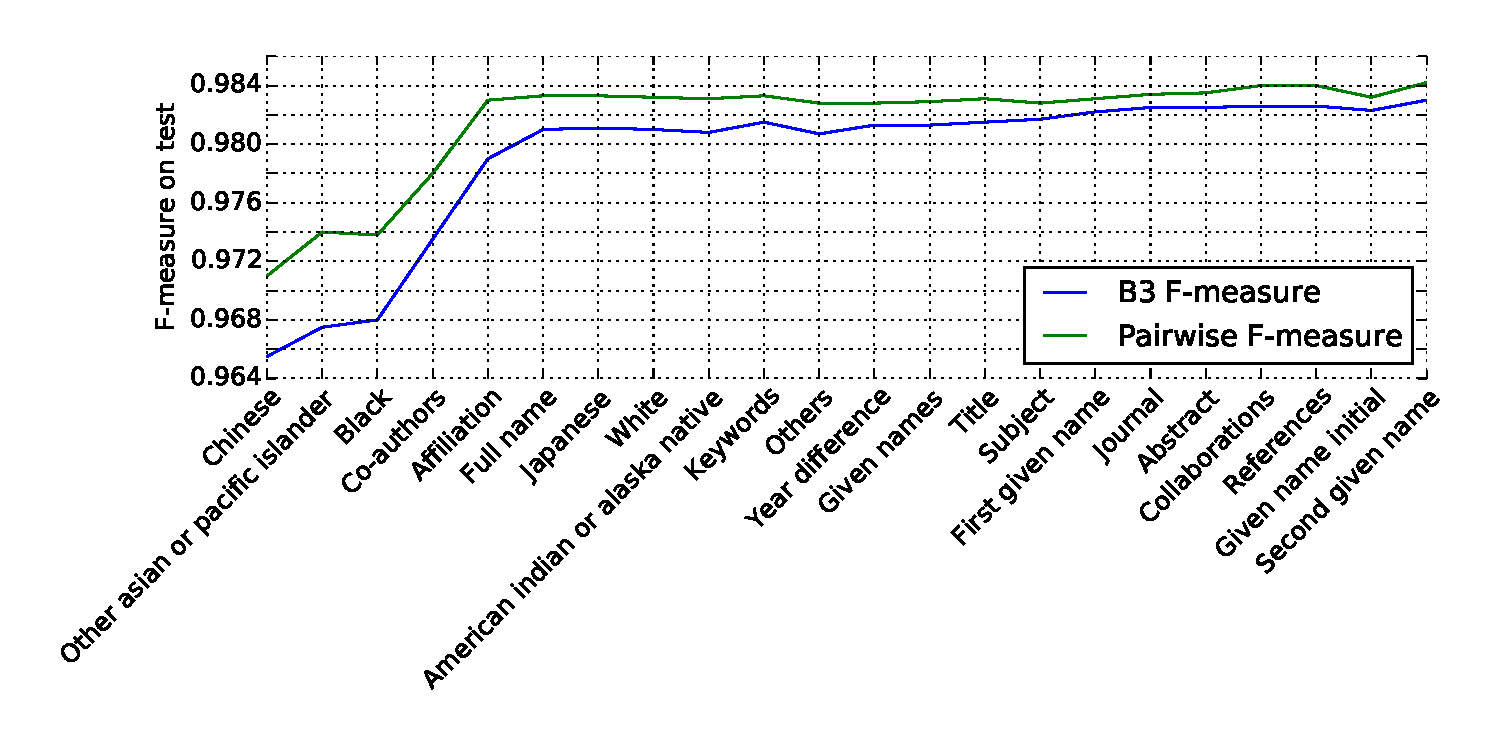
\includegraphics[width=\textwidth]{figures/fig-rfe}
\caption{The Recursive Feature Elimination scheme. The $x$ axis represents
the features removed at each step. The first results on the right represent
the performance with all 22 features used. The first results on the
left represent the performance of the algorithm with just one feature used:
\textit{Chinese}.}
\label{fig:rfe}
\end{figure}

As we can see, using only 5 features: \textit{Chinese},
\textit{Other Asian or pacific islander}, \textit{Black}, \textit{Co-authors},
and \textit{Affiliation} the algorithm performs almost as good as the one with all
the features used (resp. $0.9832$ and $0.9846$). In other words,
we can remove majority of the features and still have a well performing solution.
Moreover, this figure shows
that the algorithm makes use of the ethnicity features. The ethnicity features
were among the most important ones:

\begin{itemize}
\item{\textit{Chinese} feature was removed as the last one;}
\item{\textit{Other Asian or pacific islander} feature was removed as the last but one;}
\item{\textit{Black} feature was removed as the last but two;}
\end{itemize}


This observation can lead to a claim that our algorithm is sensitive to ethnicity. The nodes
of a tree often contain rules concerning ethnicities,
and the rest of it is built taking into account the details deriving from the
ethnicity background. With ethnicity features, the algorithm performs better
(see Table \ref{tab:15}).

\section{Comparison of clustering techniques}
Using the model, blocking and sampling from state-of-the-art we compare the linkages
criterion for the hierarchical clustering. Furthermore, we compare different
cut techniques, using the state-of-the-art algorithm as a basis.
The results are presented in Table \ref{tab:14}.


The best linkage in our case is the UPGMA.
UPGMC linkage achieves the same value of precision  as UPGMA ($0.9901$), but 
lower value of recall ($0.9686$ vs $0.9760$). Another linkage with promising
precision is WPGMC ($0.9880$), but its recall is not acceptable ($0.9486$).
A good $F_{1}$ score is also achieved by WPGMA linkage.

Our modification of semi-supervised cut choice improved noticeably the performance
from $0.9814$ to $0.9830$.

\begin{table}[H]
\caption{Comparison of performance of different clustering techniques with
the rest of the algorithm settings following the state-of-the-art.}
\centering
\begin{tabular}{|l|c c c | c c c|}
  \hline
                       & \multicolumn{3}{c|}{$\mathbf{B^{3}}$} & \multicolumn{3}{c|}{\textbf{Pairwise}}\\
  \textbf{Description} & $P$ & $R$ & $F$ & $P$ & $R$ & $F$ \\
  \hline
\hline
Clustering = UPGMA linkage & 0.9901 & 0.9760 & \textbf{0.9830}  & 0.9948 & 0.9738 & \textbf{0.9842} \\
Clustering = Single linkage & 0.9741 & 0.9603 & 0.9671  & 0.9543 & 0.9626 & 0.9584 \\
Clustering = Complete linkage & 0.9862 & 0.9709 & 0.9785  & 0.9920 & 0.9688 & 0.9803 \\
Clustering = UPGMC linkage & 0.9901 & 0.9686 & 0.9792 & 0.9950 & 0.9649 & 0.9820 \\
Clustering = WPGMC linkage & 0.9880 & 0.9486 & 0.9679 & 0.9881 & 0.9456 & 0.9664 \\
Clustering = WPGMA linkage & 0.9879 & 0.9725 & 0.9802 & 0.9920 & 0.9696 & 0.9807 \\
\hline
No cut (baseline) & 0.9024 & 0.9828 & 0.9409  & 0.8298 & 0.9776 & 0.8977 \\
Global cut & 0.9892 & 0.9737 & 0.9814  & 0.9940 & 0.9727 & 0.9832 \\
Block cut & 0.9901 & 0.9760 & \textbf{0.9830}  & 0.9948 & 0.9738 & \textbf{0.9842} \\
\hline
\end{tabular}
\label{tab:14}
\end{table}

\section{A driving example}

In order to illustrate how our methodology works we will come back to \hyperref[ex4]{Example 4}
and check how our algorithm performed. For this comparison we will use the best combined settings
with an exception of Double Metaphone blocking. With this phonetic algorithm,
both of the signatures from the example are assigned
to the same block. The first metaphones of \textit{Vaniachine} and \textit{Vanyashin} names are the
same - the output of the algorithm for each of them is \textit{FNXN}. The block of \textit{FNXN}
is small and it is not split over the first initials of the names. The only labeled signatures that
belong to it are:

\begin{itemize}

\item{217 signatures written by \textit{Vaniachine, Alexandre}}
\item{46 signatures written by \textit{Vaniachine, A.}}
\item{2 signatures written by \textit{Vaniachine, Alexandre V.}}
\item{2 signatures written by \textit{Vaniachine, A. V.}}
\item{32 signatures written by \textit{Vanyashin, A.}}
\item{15 signatures written by \textit{Vanyashin, A. V.}}

\end{itemize}

Here we can reveal that all of these signatures belong to the same author. Moreover, this
author does not have other labeled signatures in our dataset. 40 of these signatures
were a part of our training set. The name \textit{Vanyashin, A.}
or \textit{Vanyashin, A. V.} appeared on 7 out of them.

We selected one of the signatures with name \textit{Vaniachine, Alexandre} on it, and we checked
how our linkage function performed. 
For every other signature from the block we computed the probability that this and the selected
signature belong to the same author. The vast majority of the probabilities were very high.
Only 2 probabilities
out of 313 were lower than $0.5$ (these probabilities had value of $0.2865$ and $0.3929$).
The linkage function gains such confidence due to few factors. First of all, the majority
of signatures contain the surname \textit{Vaniachine}. Even if the
surnames differ, the 3-grams \textit{van} and \textit{hin} appear on both name variants.
Moreover, the author published many papers working for collaborations, where a lot
of co-authors did not change throughout the years. Finally, the author was affiliated
to the same scientific center on most of the signatures.

Our clustering created a single cluster. The signatures from the training signatures
were contained within both subtrees of the dendogram's root. Our semi-supervised strategy
chooses then to cut the tree above the root creating a single cluster. However, if the training signatures
had been contained within only one of the subtrees, the clustering would have still created
only one cluster. If few cuts result in the same $B_{3}$ score on the training subset,
the cuts that create less clusters are preferred. Moreover, even in the case of no signatures
from the training set in the block, the result would still be a single cluster.

This example shows that our algorithm effectively fixes the issue mentioned in \hyperref[ex4]{Example 4}.


\chapter{Conclusion}

We developed an author disambiguation methodology whose performance improves user experience
of the Inspire service. The algorithm
is fully integrated within the service. Moreover, it is available for other uses,
as it comes as an easy-to-use open-source library.

We compared four classifiers, six linkage functions, three techniques for sampling training pairs.
For the comparison we chose techniques that were used in related works.
Moreover, our methodology introduces novel techniques that improve the performance.
These are:
\begin{itemize}
\item{Blocking techniques based on the phonetic algorithms. These techniques make it possible
to cluster together signatures with names transliterated in various ways. Moreover
our techniques cope with signatures with multiple surnames;}
\item{Ethnicity features. These features make the algorithm sensitive to the ethnicity
of the authors;}
\item{Semi-supervised technique of choosing the cutting thresholds in dendograms blockwise.
With this technique the disambiguation is tailored to each block separately.}
\end{itemize}
In our case, the best classifier was the random forest. We observed that the pairs
that are the input of the classifier should be sampled focusing on the underrepresented
cases such as different authors who write publication under the same name. UPGMA
turned out to be the best linkage function.

In the work we discuss the problem of cluster matching and we suggest a solution based on
linear programming.

The whole algorithm described in the thesis can be run incrementally, without performing
time consuming computations over the whole dataset.

In order to popularize the idea of comparing the performance of various solutions,
we released our whole labeled dataset.

\section{Possible improvements and extensions}
While working on the solution for Inspire, we noticed that there are interesting
subproblems that still have to be investigated. Some of the possible extensions of
our pipeline include:

\begin{itemize}

\item{Improving the blocking techniques. The algorithm should be able to overcome the issue of an author
who changes his name. Such approach would have to consider more features than
just the names while the blocking is performed. A promising work could
use the advances in the field of learning representations, such as embeddings. It could
build upon a simple author embedding presented in \citep{author2vec};}

\item{Building a phonetic algorithm tailored to author disambiguation. The phonetic
algorithms used in this work for blocking do not catch all transliteration issues.
We believe it should be possible to construct an algorithm that will fare better;}

\item{Trying clustering algorithms for large datasets
that have $o(n^2)$ computational complexity. With
such algorithms the library would be significantly faster;}

\item{Investigating and evaluating the cluster matching algorithm (see Chapter \ref{sec:clustermatch});}

\item{Learning ethnicity features on datasets covering large populations. The census
dataset used in this work is small and we believe that more data points would
model the ethnicities better;}

\item{Trying our disambiguation library beyond the context of author disambiguation.
If we forget about our domain (so we do not limit ourselves to
publications and signatures) the problem that we solve is the record linkage problem.
Our library can be used for record linkage, and it might be beneficial to try it
on large labeled datasets;}

\item{Enhancing our model to accommodate feedback from Inspire users.}

\end{itemize}

\bibliographystyle{apalike}
\bibliography{bib}

\end{document}